\documentclass[a4paper]{article}

% Basic packages
\usepackage{fontspec}
\XeTeXlinebreaklocale "zh"    % 启用中文断行（XeTeX 内建，无需 xeCJK）
\XeTeXlinebreakskip = 0pt plus 1pt
\setmainfont{Songti SC}
\setsansfont{Heiti SC}
\setmonofont{Menlo}
\usepackage{amsmath, amssymb}
\usepackage{graphicx}
\usepackage[margin=2.5cm]{geometry}
\usepackage[most]{tcolorbox}
\usepackage{etoolbox}
\usepackage{listings}
\usepackage{hyperref}
\usepackage{booktabs}
\usepackage{subcaption}
\usepackage{float}

% Chinese font setup (macOS system fonts, no ctex needed)
\setmainfont{Songti SC}
\setsansfont{Heiti SC}
\setmonofont{Menlo}
\newcommand{\song}{\fontspec{Songti SC}}
\newcommand{\hei}{\fontspec{Heiti SC}}
\newcommand{\kai}{\fontspec{KaiTi}}
\newcommand{\fangsong}{\fontspec{FangSong}}

% ===== Highlight boxes =====
\newtcolorbox{knowledgebox}[1]{
    enhanced, colback=blue!5!white, colframe=blue!75!black, colbacktitle=blue!75!black,
    coltitle=white, fonttitle=\bfseries, title=#1, attach boxed title to top left={yshift=-2mm, xshift=2mm},
    boxrule=1pt, sharp corners
}

\newtcolorbox{importantbox}[1]{
    enhanced, colback=yellow!10!white, colframe=yellow!80!black, colbacktitle=yellow!80!black,
    coltitle=black, fonttitle=\bfseries, title=#1, sharp corners
}

\newtcolorbox{warningbox}[1]{
    enhanced, colback=red!5!white, colframe=red!75!black, colbacktitle=red!75!black,
    coltitle=white, fonttitle=\bfseries, title=#1, sharp corners
}

\newtcolorbox{practicebox}[1]{
    enhanced, colback=green!5!white, colframe=green!60!black, colbacktitle=green!60!black,
    coltitle=white, fonttitle=\bfseries, title=#1, sharp corners
}

% ===== Code listings =====
\lstset{
    basicstyle=\ttfamily\small,
    keywordstyle=\color{blue},
    stringstyle=\color{red!60!black},
    commentstyle=\color{green!60!black},
    breaklines=true,
    frame=single,
    numbers=left,
    numberstyle=\tiny\color{gray},
    captionpos=b,
    extendedchars=false
}

% ===== Front-page metadata =====
\newcommand{\notetitle}{CS336 Lecture 3：架构与超参数}
\newcommand{\notesubtitle}{Stanford CS336: Language Modeling from Scratch (Spring 2025)}
\newcommand{\noteauthors}{讲师：Tatsu Hashimoto, Percy Liang \quad 笔记：ZCode}
\newcommand{\notedate}{2026-07-14}
\newcommand{\videochannel}{Stanford CS336}
\newcommand{\videopublishdate}{2025 Spring}
\newcommand{\videoduration}{87 分钟}
\newcommand{\videourl}{https://www.youtube.com/watch?v=ptFiH_bHnJw}
\newcommand{\videocoverpath}{cover.jpg}

\begin{document}

% ===== Title page =====
\begin{titlepage}
\centering
{\Large 课程笔记\par}
\vspace{1.2cm}
{\huge\bfseries \notetitle\par}
\vspace{0.3cm}
{\large \notesubtitle\par}
\vspace{0.5cm}
{\large \noteauthors\par}
\vspace{0.3cm}
{\large \notedate\par}
\vspace{1.0cm}

\includegraphics[width=0.82\textwidth,height=0.40\textheight,keepaspectratio]{\videocoverpath}\par

\vfill
\begin{tcolorbox}[width=0.9\textwidth, colback=black!2!white, colframe=black!60, sharp corners]
\textbf{视频作者/频道}：\videochannel\par
\textbf{发布日期}：\videopublishdate\par
\textbf{视频时长}：\videoduration\par
\textbf{视频链接}：\href{\videourl}{\nolinkurl{\videourl}}
\end{tcolorbox}
\end{titlepage}

\tableofcontents
\newpage

%% --- 正文内容开始 ---

\section{导论：为什么这一讲要"抠细节"}

\subsection{一切你不想知道的 LM 架构与训练细节}

本讲由 Tatsu Hashimoto 主讲（Percy Liang 共同授课），标题被故意起得有些挑衅——"Everything you didn't want to know about LM architecture and training"（一切你不想知道的 LM 架构与训练细节）。Tatsu 坦言自己比起 Percy "less innovative in lecturing"，因此这一讲使用 PowerPoint 而非可执行 Python 笔记，但课程 PDF 同样可在网站上获取。

这一定调本身就传达了一个核心立场：CS336 认为大量其他课程会"spare you the details"（放过细节）的做法，恰恰是阻碍研究者真正理解大模型的根源。本讲的目标就是把这些"what should my hyperparameters be"级别的工程问题，从经验性的"凭感觉选"提升到可以据理力争、可以查文献佐证的层面。

\begin{knowledgebox}{本讲的两大主题}
\begin{itemize}
    \item \textbf{Architecture variations（架构变体）}：归一化层、激活函数、注意力变体、位置编码等组件，从 2017 年原始 Transformer 到 2025 年最新模型的演化与"趋同进化"。
    \item \textbf{Hyperparameters（超参数）}：FFN 比例、head 数量、宽深比、词表大小、初始化、正则化等，如何用证据而非拍脑袋来选择。
\end{itemize}
\end{knowledgebox}

\subsection{从原始 Transformer 到现代共识变体}

Tatsu 以一张对比图开场，把"标准 Transformer"（你在 CS224N 里学过的那种）与"你在作业里要实现的现代变体"并排放在一起。

\begin{figure}[H]
\centering
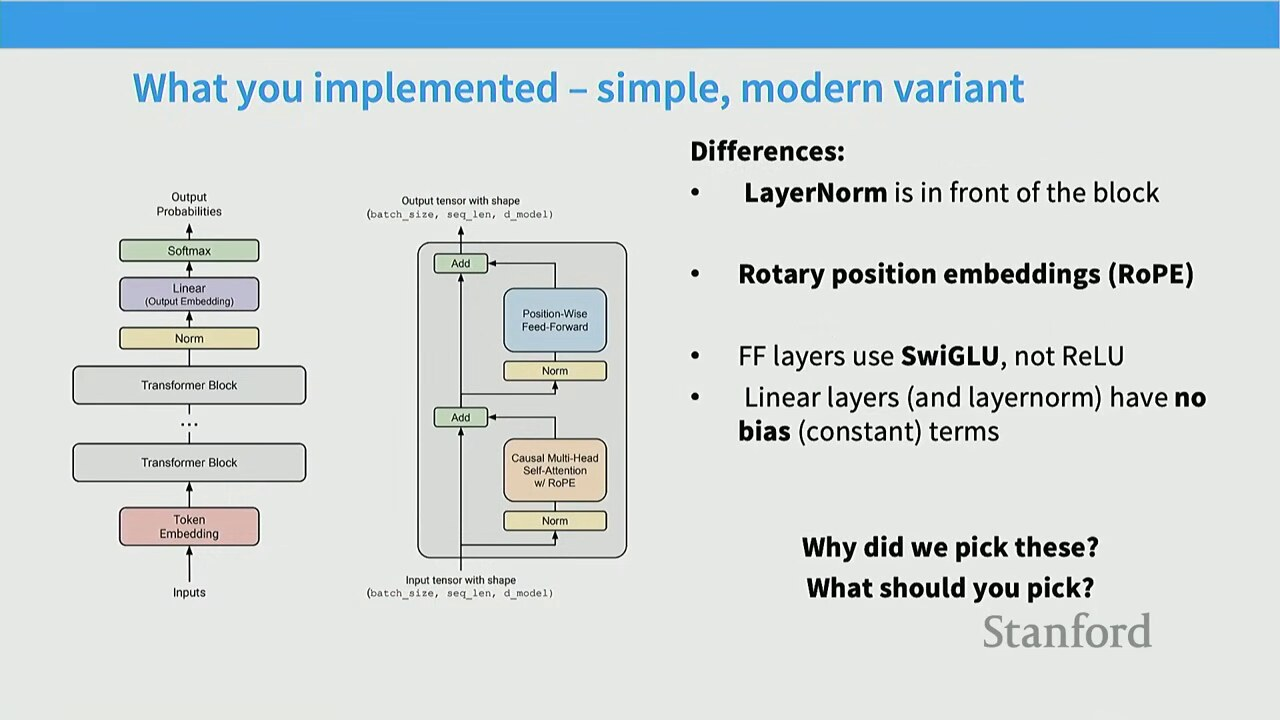
\includegraphics[width=\textwidth]{figures/fig_02_vanilla_vs_modern.jpg}
\caption{原始 Transformer 与现代共识变体的对比：norm 位置、位置编码、激活函数、bias 的差异\protect\footnotemark}
\end{figure}
\footnotetext{视频画面时间区间：00:02:15--00:02:45。}

原始 Transformer（2017，"Attention Is All You Need"）的结构：底部是 simple position embeddings，向上依次是 multi-head attention、layer norm（放在子组件\emph{之后}）、残差连接、MLP，顶部是 softmax。而 CS336 作业要求实现的"现代共识变体"已经做了至少四处关键修改。

\begin{figure}[H]
\centering
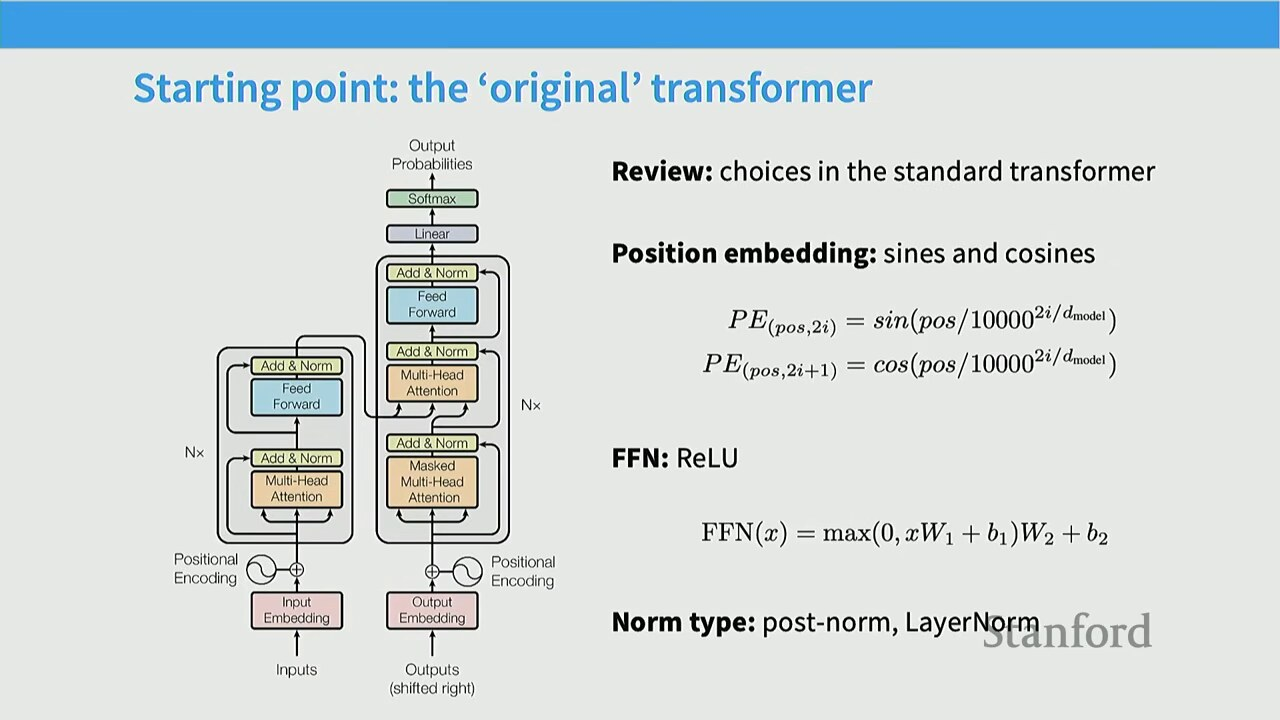
\includegraphics[width=\textwidth]{figures/fig_01_modern_variant.jpg}
\caption{"What you implemented"：现代 Transformer 变体总览（pre-norm + RoPE + SwiGLU + 无 bias）\protect\footnotemark}
\end{figure}
\footnotetext{视频画面时间区间：00:01:45--00:02:15。}

\begin{importantbox}{现代共识变体的四处关键改动}
\begin{enumerate}
    \item \textbf{Pre-norm}：把 layer norm 移到每个子组件\emph{之前}，让残差通路保持纯净的恒等映射。
    \item \textbf{Rotary Position Embedding (RoPE)}：用旋转代替加性位置编码，强制只编码相对位置。
    \item \textbf{SwiGLU 激活}：前馈层用门控线性单元（gated linear unit）替代 ReLU。
    \item \textbf{去掉 bias}：线性层不再带 bias 项。
\end{enumerate}
\end{importantbox}

Tatsu 提出一个直接的问题：为什么我们"强迫"你实现这个奇怪的变体，而不是原汁原味的 vanilla Transformer？这正是本讲要回答的核心疑问。他随后展示了一张"模型动物园"电子表格，把 2017 到 2025 年所有主流模型的架构选择铺在一张表里。

\begin{figure}[H]
\centering
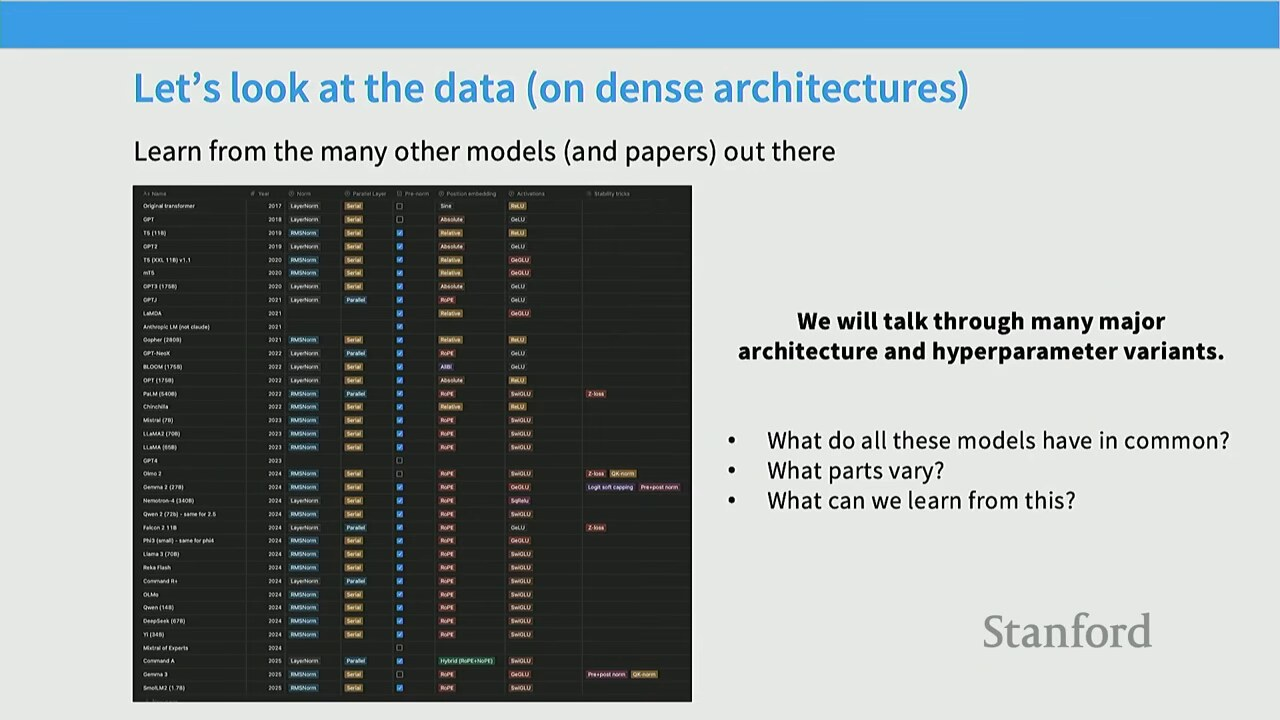
\includegraphics[width=\textwidth]{figures/fig_03_model_zoo.jpg}
\caption{模型动物园：2017→2025 各模型架构超参数对比表（OLMo 2 / Llama 3 / Gemma 3 / Qwen2.5 等）\protect\footnotemark}
\end{figure}
\footnotetext{视频画面时间区间：00:03:45--00:04:15。}

仅过去一年就有约 19 个新的 dense model 发布，许多带有"minor architecture tweaks"。一方面逐个读完这些论文"kind of annoying"，但另一方面这是一座金矿——因为并非所有模型都做同样的事，从中可以读出"convergent evolution"（趋同进化）的轨迹。例如 position embedding 这一列：早年人们尝试过 absolute、relative、RoPE、ALiBi 等各种方案，但从 2023 年起几乎所有人都收敛到了 RoPE。

\begin{figure}[H]
\centering
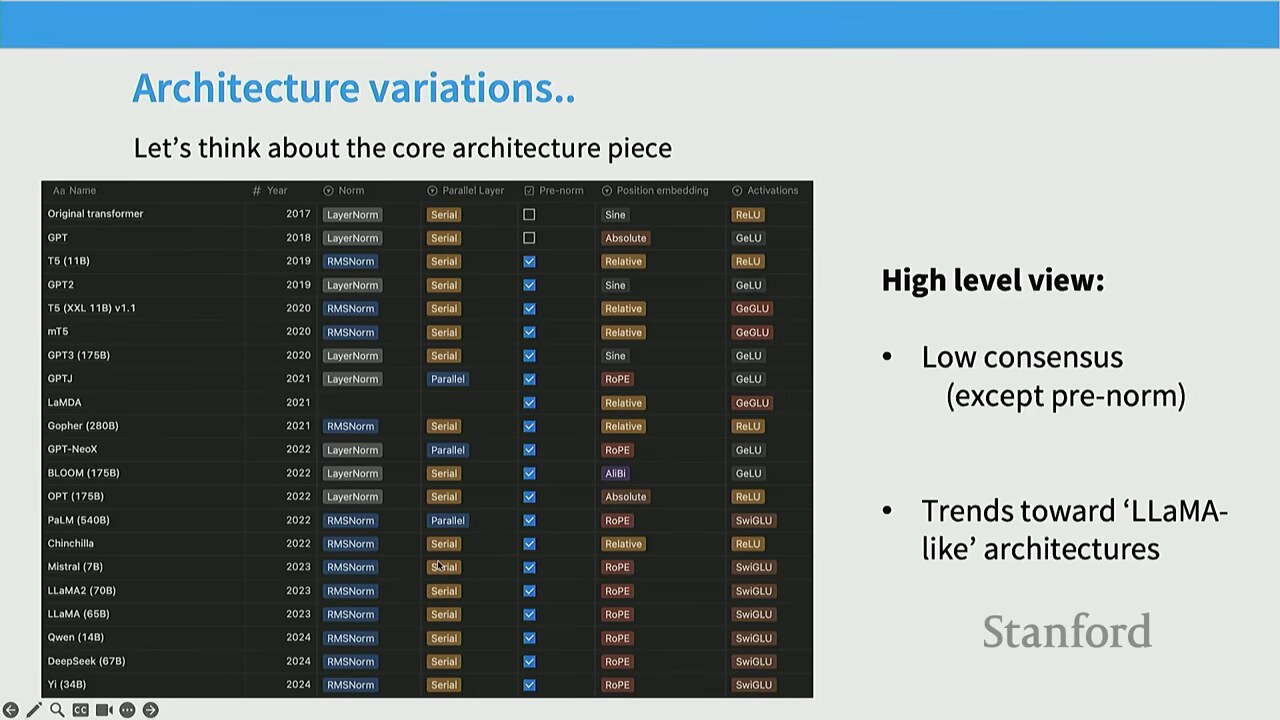
\includegraphics[width=\textwidth]{figures/fig_04_arch_variations.jpg}
\caption{架构组件变迁表：norm 类型/位置、position embedding、activation 在各模型间呈现"低共识"\protect\footnotemark}
\end{figure}
\footnotetext{视频画面时间区间：00:05:15--00:05:45。}

\begin{knowledgebox}{本讲的方法论：从他人的经验中学习}
整门课的主题是"best way to learn is hands-on experience"（最好的学习方式是亲手做），但本讲是个例外——因为我们不可能把所有这些 Transformer 都训练一遍。所以本讲的主题是"learn from the experience of others"（从他人的经验中学习）：用一种近乎进化生物学的分析方式，读文献、看趋势、辨真伪。
\end{knowledgebox}

\section{架构变体之一：归一化层}

\subsection{Pre-norm vs Post-norm：一场被反转的争论}

Tatsu 认为，归一化层是"基本上所有人都同意、而且几乎从一开始就同意"的一个设计选择——pre-norm 优于 post-norm。但这个共识的形成有一段曲折的历史。

\begin{figure}[H]
\centering
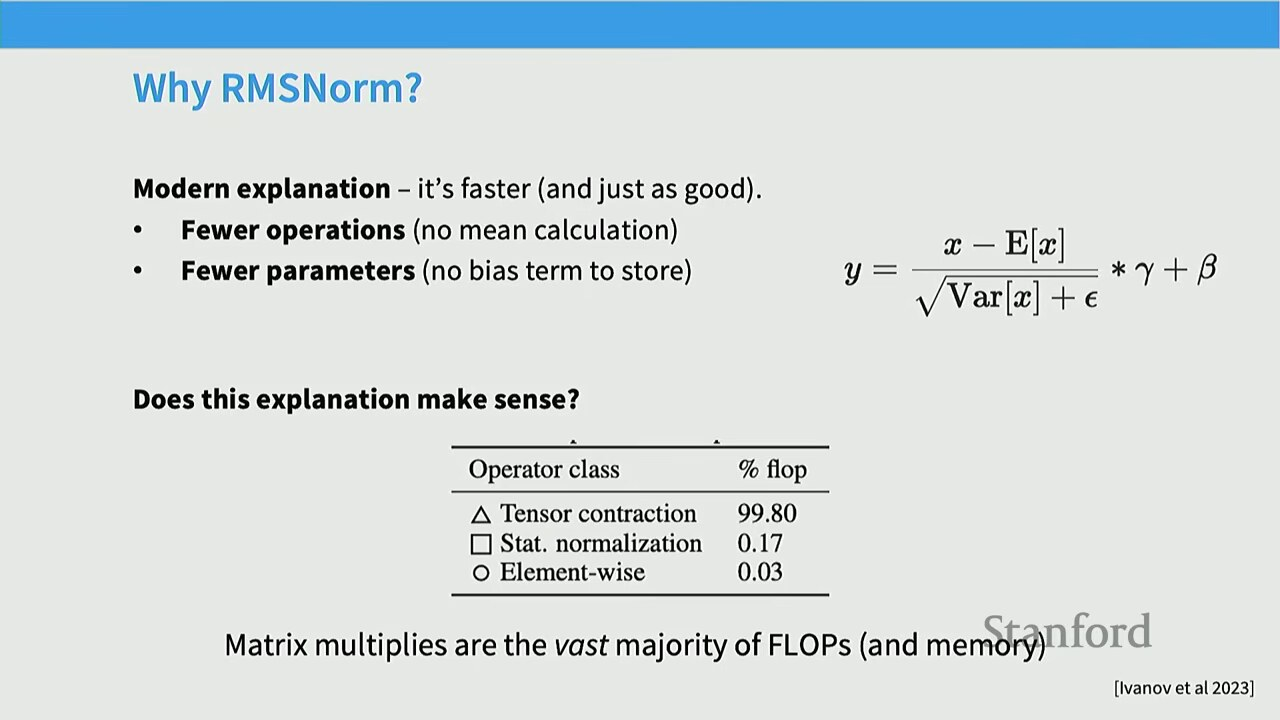
\includegraphics[width=\textwidth]{figures/fig_07_norm_placement.jpg}
\caption{归一化位置对比图：post-norm（块后）与 pre-norm（块前）的架构并排\protect\footnotemark}
\end{figure}
\footnotetext{视频画面时间区间：00:13:15--00:13:45。}

原始 Transformer 论文用的是 post-norm：你在残差流里做完 multi-head attention、加回残差，\emph{然后}才 layer norm；MLP 同理。也就是说 norm 位于残差主路上。而 pre-norm 把 norm 移到子组件的\emph{输入}端，让残差流本身保持一条干净的恒等通路。

\begin{figure}[H]
\centering
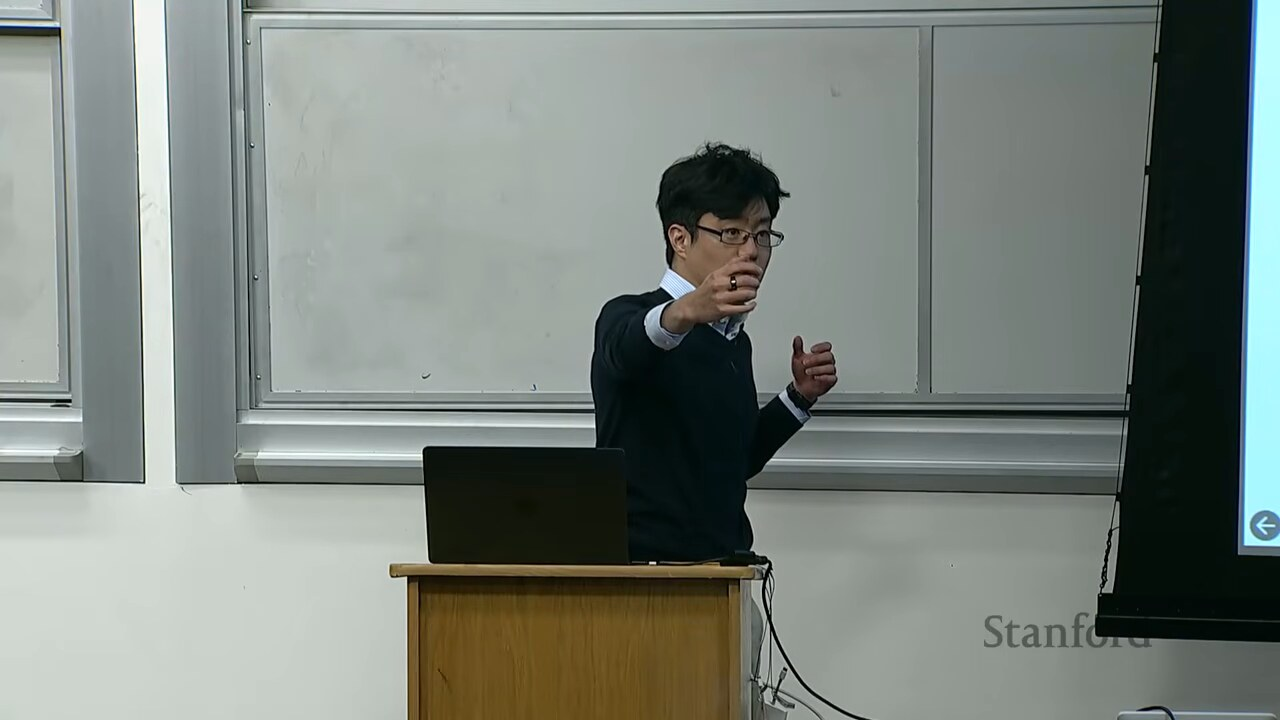
\includegraphics[width=\textwidth]{figures/fig_06_prenorm_vs_postnorm.jpg}
\caption{PreNorm vs PostNorm：归一化放在残差块前还是后，残差通路是否被 norm 干扰\protect\footnotemark}
\end{figure}
\footnotetext{视频画面时间区间：00:10:45--00:11:15。}

支持 pre-norm 的早期论文（Salazar \& Yen 2020、Xiong 2020 等）几乎都会展示同一类对比图：如果用 pre-norm 并配合其他稳定性技巧，就可以\emph{去掉 learning rate warm-up}，效果与"post-norm + 精心 warm-up"相当甚至更好。一种解释是\textbf{梯度衰减（gradient attenuation）}：pre-norm 下各层梯度规模保持恒定，而 post-norm 在没有 warm-up 时梯度会"blow up"。

\begin{figure}[H]
\centering
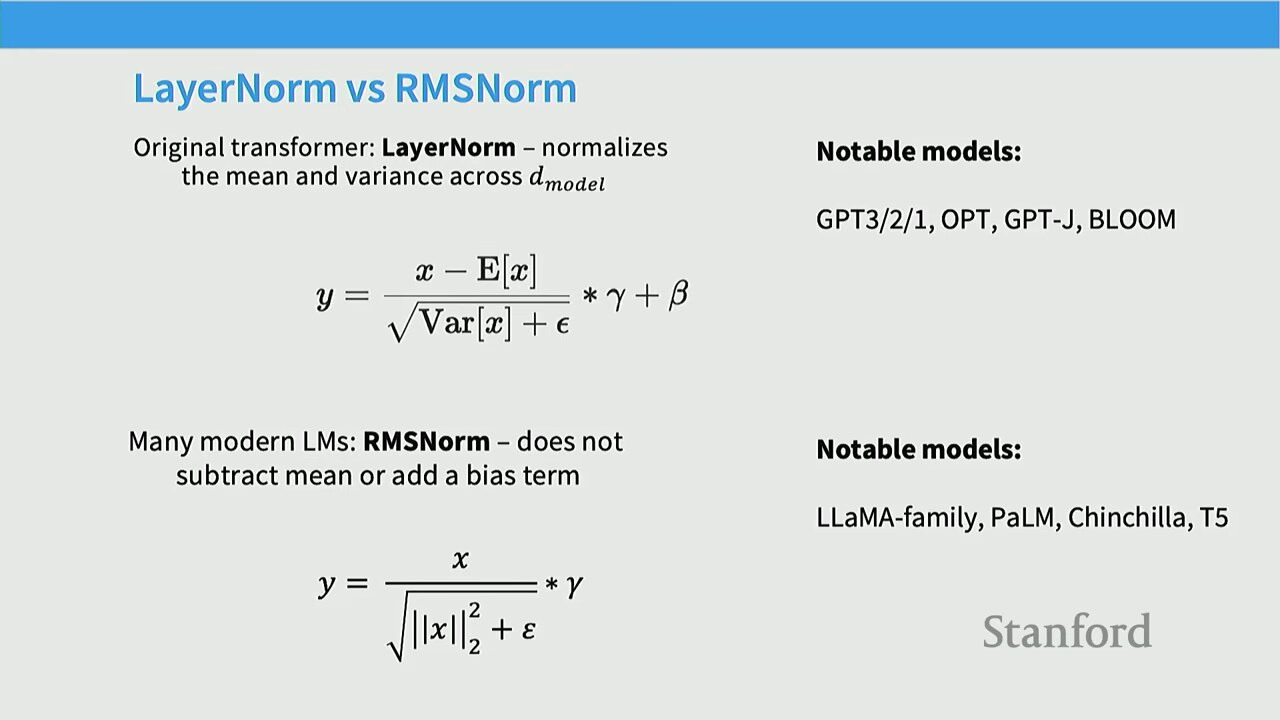
\includegraphics[width=\textwidth]{figures/fig_24_norm_debate.jpg}
\caption{归一化位置争论：post-norm 早期更好但需 warmup，pre-norm 更稳定\protect\footnotemark}
\end{figure}
\footnotetext{视频画面时间区间：00:11:45--00:12:15。}

\begin{warningbox}{为什么把 norm 放在残差流里"不好"？}
有学生在课上提问：为什么 layer norm 在 residual stream 里是坏的？Tatsu 给出了一个直觉性的（而非严格证明的）解释：残差连接提供了一条从网络顶部几乎直达底部的\textbf{恒等映射（identity connection）}。这对训练极深网络至关重要——它让梯度反向传播变得很容易（对比 LSTM、状态空间模型那种梯度难以长程传播的结构）。而把 layer norm 塞进残差通路中间，就会"mess with"这种干净的梯度行为。这正是为什么大家形成了"iron rule"（铁律）：norm 一定要放在残差流\emph{之外}。
\end{warningbox}

Tatsu 还提到一个有趣的考古发现：OPT 350M 是个"orphaned"的例外，疑似 Meta 在训练时"kind of messed that one up"用了 post-norm。这成了他做架构普查时的一个 fun find。

\subsubsection{新近的"double norm"变体}

Pre-norm 主导了很久，但最近（"I don't think this existed when I gave this lecture last year"）出现了新变化。有人问：为什么 norm 只能放在前面，不能放在 FFN 之后？当然可以。Grok 和 Gemma 2 都采取了"前后都放 norm"的策略——layer norm 既在每个子组件之前、也在之后。Gemma 2 则只在 attention 和 FFN \emph{之后}放 norm。这被称为（Tatsu 临时命名的）"double norm"。有评估显示这种方式在更大模型上训练更稳定、更友好。

\subsection{LayerNorm 的数学：从公式说起}

在讨论 norm 类型之前，Tatsu 先给了一个 LayerNorm 的"primer"（入门回顾）。

\begin{figure}[H]
\centering
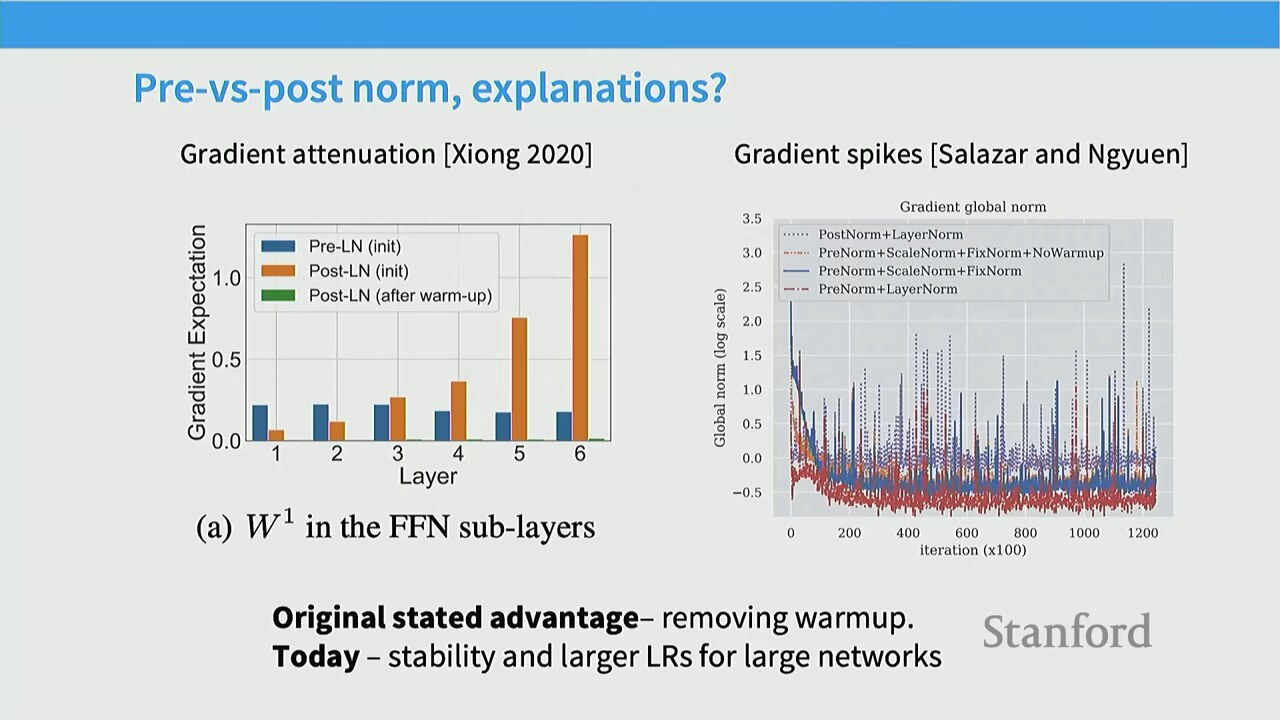
\includegraphics[width=\textwidth]{figures/fig_05_layernorm_primer.jpg}
\caption{Normalization layers primer：LayerNorm 公式（减均值除标准差再仿射变换 $\gamma/\beta$）\protect\footnotemark}
\end{figure}
\footnotetext{视频画面时间区间：00:08:15--00:08:45。}

LayerNorm 的核心思想是：对进入的激活 $x$，先减去经验均值，再除以标准差（加一个小 $\epsilon$ 防止除零），最后用可学习的 $\gamma$ 缩放、$\beta$ 平移。

\[
\mathrm{LayerNorm}(x) = \gamma \cdot \frac{x - \mathbb{E}[x]}{\sqrt{\mathrm{Var}[x] + \epsilon}} + \beta
\]

\begin{itemize}
    \item $x$：当前 token 的激活向量（对每个 token 独立地、在其特征维度上做归一化）。
    \item $\mathbb{E}[x], \mathrm{Var}[x]$：该 token 激活的经验均值与方差（沿特征维计算）。
    \item $\epsilon$：防除零的小常数（如 $10^{-5}$）。
    \item $\gamma, \beta$：可学习的逐特征缩放与平移参数（gain 与 bias）。
\end{itemize}

直觉是：先把激活"标准化"到均值 0、方差 1，再让网络自己决定把它移到哪个工作点。许多模型用了这个公式且效果不错。

\subsection{RMSNorm：更快且同样好}

但许多模型已经迁移到了 \textbf{RMSNorm}——这是又一个"consensus change"（共识性改动），几乎所有最新模型都改用 RMSNorm。

\begin{figure}[H]
\centering
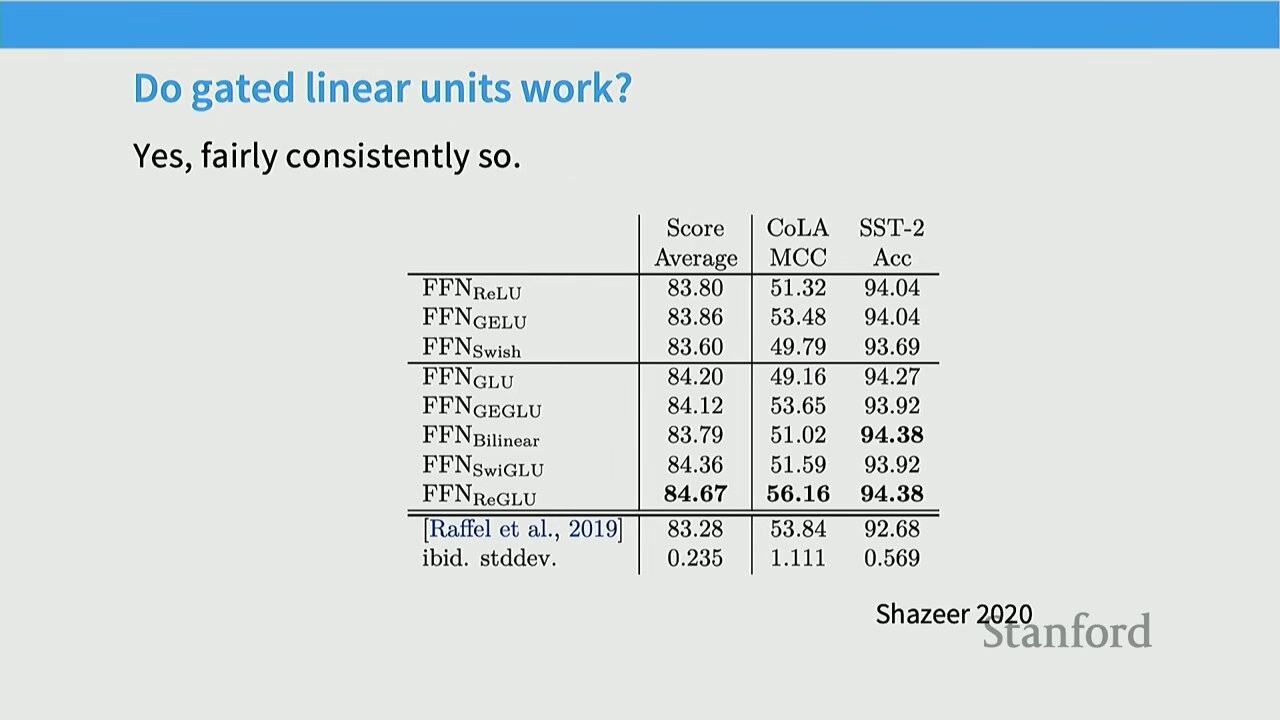
\includegraphics[width=\textwidth]{figures/fig_08_rmsnorm.jpg}
\caption{RMSNorm：去掉均值减法、仅用 RMS 归一化且无 bias，参数更少、速度快、已成主流\protect\footnotemark}
\end{figure}
\footnotetext{视频画面时间区间：00:25:45--00:26:15。}

RMSNorm 做的事情很简单：\textbf{去掉均值调整}（不减均值），也\textbf{不加 bias 项} $\beta$，只用 RMS（root mean square）做归一化。

\[
\mathrm{RMSNorm}(x) = \gamma \cdot \frac{x}{\sqrt{\frac{1}{d}\sum_{i=1}^{d} x_i^2 + \epsilon}}
\]

\begin{itemize}
    \item $x \in \mathbb{R}^d$：当前 token 的激活向量。
    \item 分母 $\sqrt{\frac{1}{d}\sum_i x_i^2}$：激活的 RMS（均方根），替代了 LayerNorm 里的标准差。
    \item $\gamma$：可学习的逐特征缩放（\textbf{没有} $\beta$ 平移项）。
\end{itemize}

Llama 家族、PaLM、Chinchilla、T5 都已迁移到 RMSNorm。理由有两层：

\begin{enumerate}
    \item \textbf{效果不差}：训练出来和 LayerNorm 一样好（"it doesn't really make a difference"）。
    \item \textbf{更快}：不减均值意味着更少的运算；不加 $\beta$ 意味着更少的参数需要从内存搬运到计算单元。
\end{enumerate}

\begin{knowledgebox}{为什么"省一点点运算"也值得？——内存搬运才是关键}
这里有一个反直觉但极其重要的工程洞察。你可能记得 224N 里讲过"只有矩阵乘法决定运行时间"。如果只看 FLOPs，Tensor contraction（矩阵乘）占了 Transformer 的 \textbf{99.8\%} FLOPs，而 softmax、layer norm 这些归一化操作只占 \textbf{0.17\%} FLOPs——省下 0.17\% 似乎微不足道。

但 \textbf{FLOPs 不是唯一要优化的资源}。根据 Ivan Anselm 2023 那篇"Memory Movement Is All You Need"风格的 profiling 论文：那些只占 0.17\% FLOPs 的归一化操作，竟然占了 \textbf{25\% 的运行时间}！原因正是它们仍然要搬运大量内存。所以在架构设计里，"减少内存搬运"和"减少 FLOPs"同等重要——这个主题会在后续 systems 讲座里反复出现。
\end{knowledgebox}

Neubig et al. 2020 的消融实验直接量化了 RMSNorm 的收益：vanilla Transformer 每秒 3.5 步，换 RMSNorm 后提升到 3.68 步——不算巨大，但"in some sense for free"，而且最终 loss 还更低。win-win。

\subsection{去掉 Bias：稳定性的隐性收益}

最后一个与 norm 同源的主题：\textbf{现代 Transformer 基本都不用 bias 项}。原始 Transformer 的 FFN 是 $\mathrm{ReLU}(xW_1 + b_1)W_2 + b_2$，而现在大多数实现直接把 bias 全部删掉，只留纯矩阵乘。

\[
\text{原始 FFN:} \quad \mathrm{ReLU}(x W_1 + b_1) W_2 + b_2
\qquad
\text{现代 FFN:} \quad \mathrm{SwiGLU}\text{ 变体，无 bias}
\]

理由同样是两层：(1) 性能与带 bias 时一样好，"matrix multiplies are apparently all that you need"；(2) 更隐蔽但更重要的一点是\textbf{优化稳定性}——Tatsu 坦言自己"don't have the deepest understanding of why bias terms are particularly bad for stability"，但有非常清晰的实证观察：丢掉 bias 往往能稳定最大规模网络的训练。

\begin{practicebox}{三条"铁律"小结}
\begin{itemize}
    \item \textbf{铁律一}：norm 一定要在残差流\emph{之外}（pre-norm 或 double norm），获得干净的恒等残差通路与稳定训练。
    \item \textbf{铁律二}：几乎所有人都用 RMSNorm（参数更少、内存搬运更少、效果不差）。Cohere 的 Command A / R+ 是少数仍用 LayerNorm 的例外。
    \item \textbf{铁律三}：广泛地丢掉 bias 项。
\end{itemize}
\end{practicebox}

有学生问：这些细节里有没有更"future-proof"（经得起时间检验）的通用教训？Tatsu 给出了三条可推广的认识：(1) 直接的恒等残差映射在许多架构族里都被证明有效；(2) 不让激活在 scale 上漂移（即 norm 的作用）对训练稳定性极其有效；(3) 必须认真考虑架构对 systems 组件（内存、并行）的影响。

\section{架构变体之二：激活函数与门控}

\subsection{激活函数的"动物园"}

接下来是激活函数。Tatsu 自嘲说这"exactly the kind of thing I didn't originally want to learn when I got into deep learning"——他曾觉得"我不关心激活函数，反正都能训练"。但事实证明 SwiGLU 和各种 GLU 变体\emph{确实}稳定地更好，所以"it really does matter, unfortunately, for both you and me"。

\begin{figure}[H]
\centering
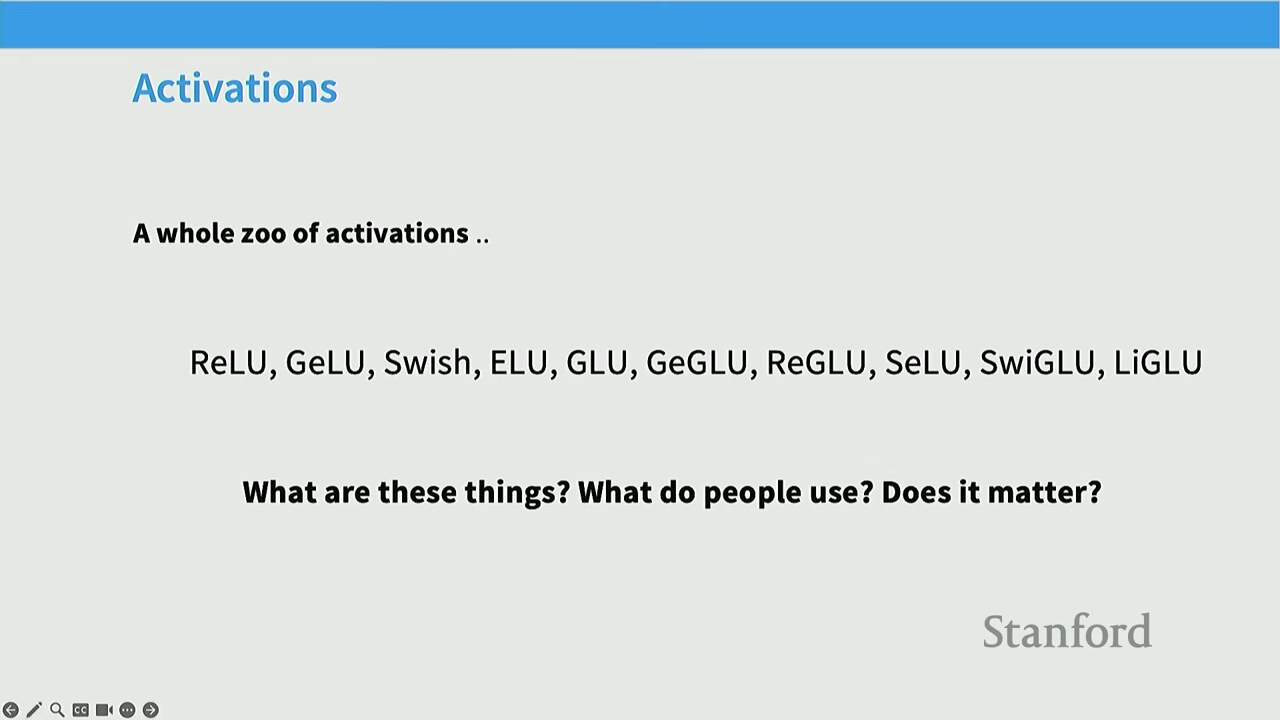
\includegraphics[width=\textwidth]{figures/fig_09_activation_relu.jpg}
\caption{激活函数：ReLU 的历史（源自 CNN）与曲线，及其在 Transformer 中的沿用\protect\footnotemark}
\end{figure}
\footnotetext{视频画面时间区间：00:19:45--00:20:15。}

先回顾最基础的两个：

\[
\text{ReLU:} \quad \mathrm{ReLU}(x) = \max(0, x)
\qquad
\text{GELU:} \quad \mathrm{GELU}(x) = x \cdot \Phi(x)
\]

\begin{itemize}
    \item $\mathrm{ReLU}(x) = \max(0,x)$：最古老的激活，来自 CNN 时代，原始 Transformer 也用它。MLP 写成 $\mathrm{ReLU}(xW_1)W_2$（此处已省略 bias）。
    \item $\mathrm{GELU}(x) = x \cdot \Phi(x)$：Gaussian Error Linear Unit，把线性项与高斯 CDF $\Phi(x)$ 相乘。形状像 ReLU 但在 0 附近有一段平滑的"小鼓包"，更可微。GPT-1/2/3、GPT-J 都用 GELU。
\end{itemize}

\subsection{门控线性单元（GLU）与 SwiGLU}

但几乎所有 2023 年之后的模型都换成了\textbf{门控线性单元（gated linear unit, GLU）}变体。核心思想：不再只做"线性 + 非线性"，而是用另一个线性投影的结果去\emph{逐元素门控}中间隐层。

\begin{figure}[H]
\centering
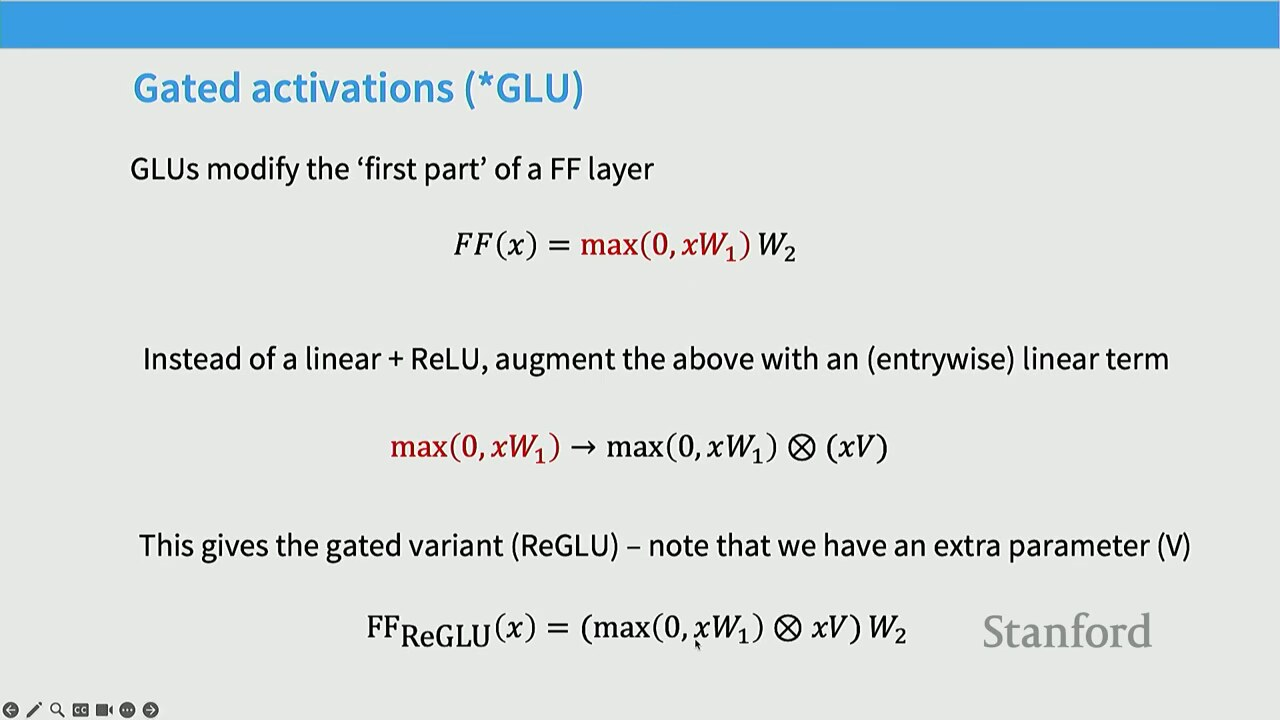
\includegraphics[width=\textwidth]{figures/fig_10_swiglu.jpg}
\caption{SwiGLU/门控线性单元：FFN 用两路投影 + SiLU 门控 + 缩放因子，配 FFN ratio\protect\footnotemark}
\end{figure}
\footnotetext{视频画面时间区间：00:22:15--00:22:45。}

把原始 ReLU FFN $\mathrm{ReLU}(xW_1)W_2$ 改造为门控版本：

\[
\mathrm{GLU}(x) = \big( x W_1 \big) \odot \sigma(x V) \quad\text{然后}\quad \mathrm{FFN}(x) = \big[\mathrm{GLU}(x)\big] W_2
\]

\begin{itemize}
    \item $x W_1$：把输入投影到隐层（"主路"）。
    \item $x V$：\textbf{额外的}门控投影，$V$ 是新增的参数矩阵。
    \item $\odot$：逐元素相乘（element-wise gating）。
    \item $\sigma(\cdot)$：门控的非线性——换成不同函数就得到不同变体：
    \begin{itemize}
        \item $\sigma = \mathrm{GELU}$ $\Rightarrow$ \textbf{GeGLU}（T5v1.1、Gemma 2/3 用）。
        \item $\sigma = \mathrm{Swish} = x \cdot \mathrm{sigmoid}(x)$ $\Rightarrow$ \textbf{SwiGLU}（Llama、PaLM 等用）。
    \end{itemize}
    \item $W_2$：把门控后的隐层投影回 $d_{\mathrm{model}}$。
\end{itemize}

\begin{importantbox}{门控（gating）是一条可推广的架构经验}
Tatsu 把"门控"列为继残差连接、layer norm 之后的第三条"generalizable architecture lesson"。门控在 Transformer 里反复出现并稳定有效。但要注意：\textbf{GLU 不是好模型的必要条件}——GPT-3 没用 GLU；最近的 Neotron 340B 用 squared ReLU，Falcon 211B 用普通 ReLU，都是高性能模型。证据只是指向 SwiGLU/GeGLU 有\emph{稳定的}小幅提升，所以作业要求你实现它。
\end{importantbox}

\subsubsection{Swish 的非单调性会是个问题吗？}

有学生提了一个很好的问题：Swish（以及 GELU）在某个负值区间是\emph{单调递减}的，这难道不会让梯度下降"走反方向"吗？Tatsu 的回答很务实：理论上你可能担心激活被"trap"在零点，但实践中优化器通常用很高的学习率加 momentum，激活"all over the place"，那个小小的负区间片段其实影响不大。

另一个关于"Swish/GELU 的 CDF 涉及平方项、可微性是否拖慢训练"的问题，Tatsu 和学生一起得出更准确的答案：\textbf{真正重要的是内存压力}，而门控前后的 element 数量相同，所以额外的计算开销可忽略，内存搬运量也不变。

\subsection{Serial vs Parallel Layers}

最后一个架构变体是\textbf{串行 vs 并行层}。标准 Transformer block 是串行的：先做 attention，结果传给 MLP，再传下去。但有些模型（GPT-J 首创，PaLM 在大尺度上推广）改成\textbf{并行层}：attention 和 MLP 同时从上一层的 $x$ 计算，结果相加后进入残差流。

\[
\text{Serial:} \quad x \to \mathrm{Attn} \to \mathrm{MLP} \to x'
\qquad
\text{Parallel:} \quad x' = x + \mathrm{Attn}(x) + \mathrm{MLP}(x)
\]

并行的动机是\textbf{系统效率}：可以把 layer norm 和矩阵乘 fuse 在一起，提升 GPU 利用率，便于在大规模 GPU 上并行。理论上串行更"expressive"（两次复合而非一次相加），但并行的系统收益让人愿意做这个交易。不过最近一年串行层又重新流行，只有 Cohere Command A/R+ 和 Falcon 11B 等少数模型仍用并行层。

\section{架构变体之三：位置编码与 RoPE}

\subsection{从绝对到相对：位置编码的演化}

位置编码是架构组件里"最有趣"的一块，因为在 LM 早期人们尝试了五花八门的方案，直到最近才收敛。

\begin{figure}[H]
\centering
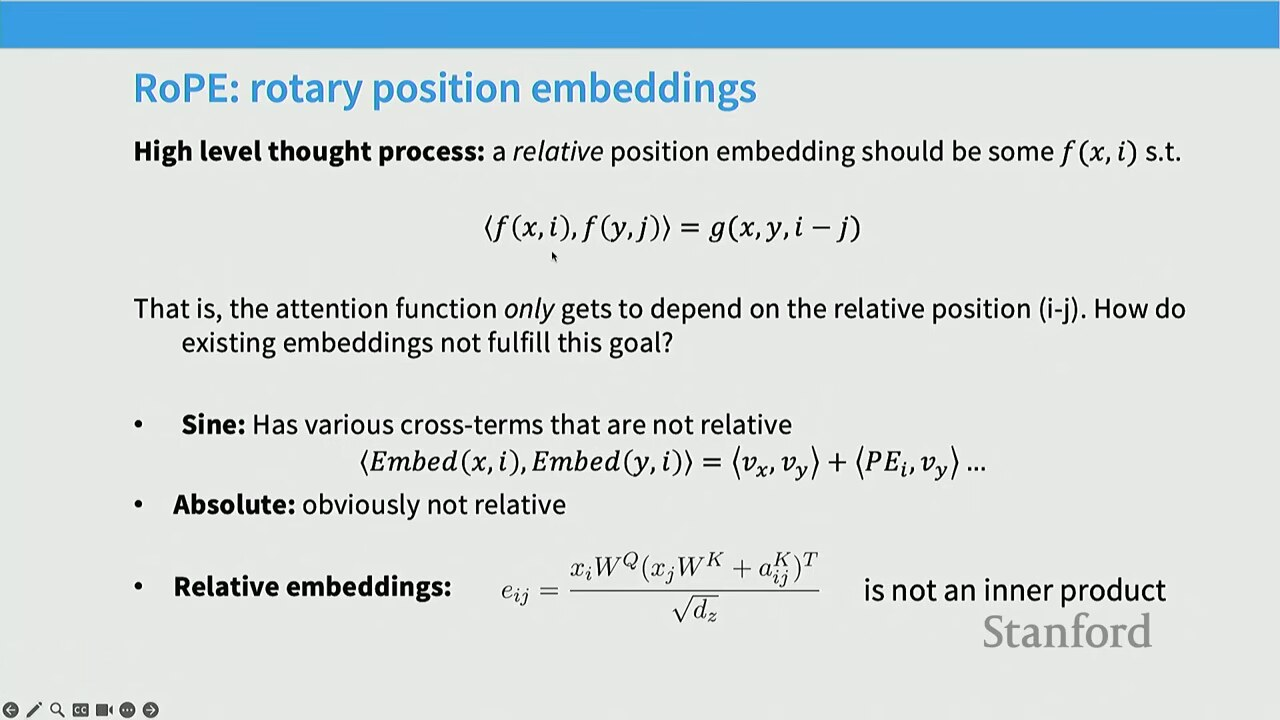
\includegraphics[width=\textwidth]{figures/fig_11_rope_intro.jpg}
\caption{Rotary Position Embedding 总览：通过旋转 query/key 向量编码相对位置\protect\footnotemark}
\end{figure}
\footnotetext{视频画面时间区间：00:33:45--00:34:15。}

Tatsu 把方案分为四类：

\begin{itemize}
    \item \textbf{Sinusoidal（正余弦）}：原始 Transformer 的 sine/cosine 位置编码。
    \item \textbf{Absolute（绝对）}：GPT、OPT 等，直接学一个位置向量加到 embedding 上。
    \item \textbf{Relative（相对）}：T5、Gopher，把相对位置向量加到 attention 计算里。
    \item \textbf{RoPE}：旋转位置编码，现已\emph{几乎统一}整个领域（GPT-J 首倡）。
\end{itemize}

RoPE 的出发点是一个原则性要求：\textbf{真正重要的应该是相对位置}。形式化地，我们希望存在一个 embedding 函数 $f$，使得任意两个 token 的内积只依赖它们的\emph{内容}与\emph{位置差}：

\[
\langle f(x_i, i),\; f(y_j, j) \rangle = g(x, y, i-j)
\]

\begin{itemize}
    \item $f(x_i, i)$：把词 $x$ 在位置 $i$ 编码成的向量。
    \item $g(x, y, i-j)$：某个只依赖两词内容 $x, y$ 与\emph{位置差} $i-j$ 的函数。
    \item 这个约束强制了\textbf{绝对位置不变性}（absolute-position invariance）：注意力只关心两个词相距多远，而不关心它们绝对在哪。
\end{itemize}

Tatsu 快速检验了前三种方案：sinusoidal 会产生非相对的交叉项（泄漏绝对位置）；absolute 顾名思义就不是相对的；relative 虽然是相对的，但它作用在 attention 的加性偏置上，\emph{不是}内积形式，违反了上述约束。而 RoPE 的关键观察是：\textbf{内积对任意旋转是不变的}——所以用旋转来编码位置就能天然满足这个约束。

\subsection{RoPE 的几何直觉与数学}

\begin{figure}[H]
\centering
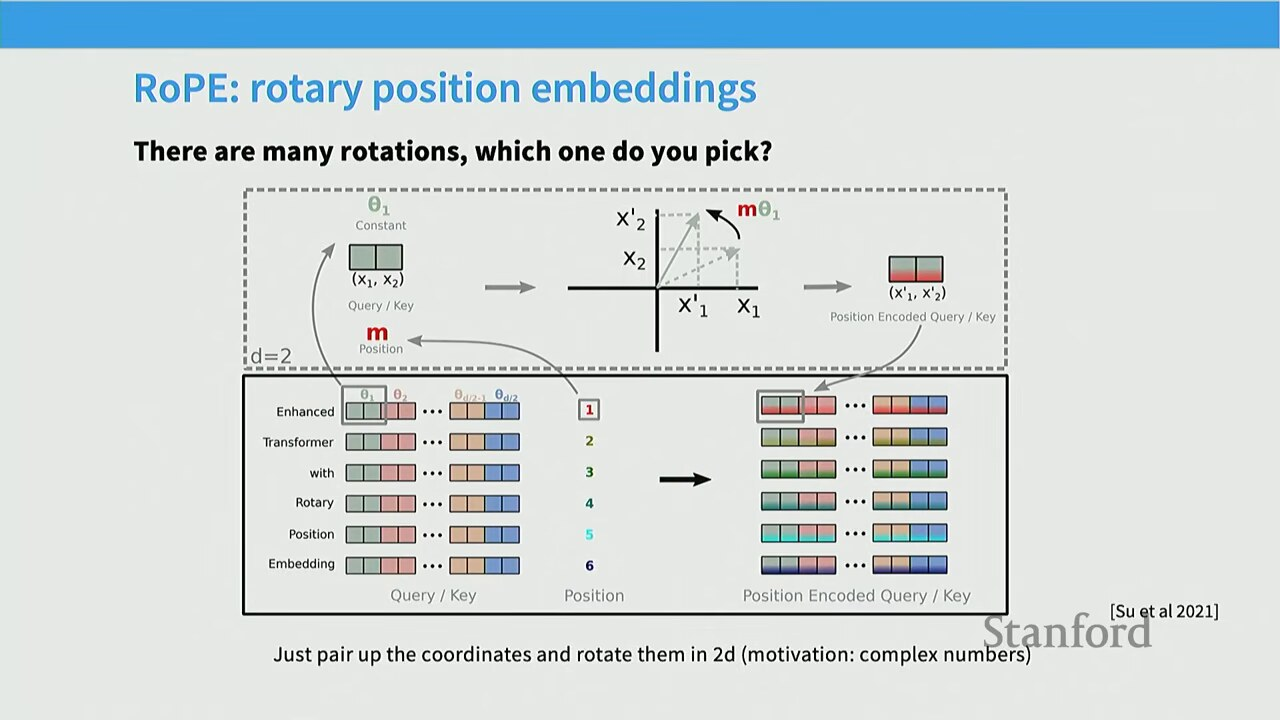
\includegraphics[width=\textwidth]{figures/fig_12_rope_rotation.jpg}
\caption{RoPE 数学推导：旋转矩阵 $R_m$ 作用于 $q/k$，内积仅依赖相对位置 $(m-n)$\protect\footnotemark}
\end{figure}
\footnotetext{视频画面时间区间：00:36:15--00:36:45。}

Tatsu 用 2D 例子讲直觉：假设 "we" 的 embedding 是某个箭头，"no" 是另一个箭头。编码序列 "we know" 时，"we" 在位置 0（不转），"no" 在位置 1（转 1 个单位角度）。换到 "we'll know" 时，"we" 转到位置 2，"no" 转到位置 3——但两者的\emph{相对夹角}不变，所以内积（只看相对夹角）也被保持。这就是 RoPE 的核心：\textbf{按位置旋转向量，旋转角度由位置决定，内积自然只反映相对距离}。

在高维空间里，RoPE 的做法是把 $d$ 维向量切成 $d/2$ 个二维块，每个块用不同的频率 $\theta$ 旋转：

\[
R_m = \mathrm{blockdiag}\!\left(
\begin{pmatrix} \cos m\theta_1 & -\sin m\theta_1 \\ \sin m\theta_1 & \cos m\theta_1 \end{pmatrix},
\dots,
\begin{pmatrix} \cos m\theta_{d/2} & -\sin m\theta_{d/2} \\ \sin m\theta_{d/2} & \cos m\theta_{d/2} \end{pmatrix}
\right)
\]

\begin{itemize}
    \item $R_m$：位置 $m$ 对应的块对角旋转矩阵，作用在 query/key 上。
    \item $\theta_k$：第 $k$ 个二维块的旋转\emph{基频}（base frequency）——类似 sinusoidal 编码，有的块转得快（捕获近距离高频信息），有的转得慢（捕获远距离低频信息）。
    \item $m$：token 的绝对位置。注意 $R_m$ 只依赖 $m$ 与固定的 $\theta$，\textbf{不含可学习参数}。
\end{itemize}

于是 query 和 key 分别被旋转：$\tilde q = R_m q$，$\tilde k = R_n k$。由于旋转保内积的相对性：

\[
\langle \tilde q, \tilde k \rangle = \langle R_m q, R_n k \rangle = q^\top R_m^\top R_n k = q^\top R_{n-m} k = g(q, k, m-n)
\]

\begin{itemize}
    \item $R_m^\top R_n = R_{n-m}$：旋转矩阵的群性质——两个旋转的复合等于一个差值旋转。
    \item 最终内积只依赖位置差 $m-n$ 与内容 $q, k$，完美满足前面的约束 $g(q,k,m-n)$。
\end{itemize}

\begin{warningbox}{RoPE 不是加在底部的！}
一个容易混淆的关键点：RoPE \textbf{不在 embedding 层加}，而是\emph{在 attention 层内、对 query 和 key 做旋转}。也就是说，每当你要算 attention，就在生成 Q、K 之后、计算 $QK^\top$ 之前，介入这个旋转操作。V 不旋转。这是强制"只编码相对位置"的必要条件——如果加在底部，信息会沿残差流"泄漏"成绝对位置。
\end{warningbox}

\subsubsection{关于 $\theta$ 与训练的几个问答}

学生的几个问题澄清了细节：

\begin{itemize}
    \item \textbf{各模型的旋转速率一致吗？} 不完全一致，$\theta$ 有些变化。
    \item \textbf{$\theta$ 是超参数还是训练出来的？} 都不是——它是\textbf{固定}的频率调度（类似 sinusoidal 的思路），用来覆盖不同频率范围，不需要学习。
    \item \textbf{旋转会不会给训练带来困难？} 不会。因为 $\theta$ 固定、$m$ 固定，$R_m$ 本质上就是一个\emph{固定的矩阵}乘到向量上，并不涉及对三角函数求导。如果去学习 $\theta$ 才可能有麻烦。
\end{itemize}

\begin{knowledgebox}{RoPE 为何"赢了"位置编码之战}
Tatsu 强调他周末把这 19 篇新论文都过了一遍，\emph{基本所有}模型现在都用 RoPE。原因有二：(1) RoPE 衍生出了大量\textbf{上下文长度外推}算法（如 NTK-aware、YaRN 等），是现代生产级 LM 处理长上下文的关键基础设施；(2) 即便在小尺度、小上下文下，RoPE 也经验性地很有效。所以它在"position embedding battle"中胜出。
\end{knowledgebox}

\section{超参数：用证据而非拍脑袋做选择}

\subsection{设计问题清单：哪些超参数真正重要}

进入第二大主题——超参数。Tatsu 的核心论点是：真正在成功模型之间被改动的超参数\emph{其实很少}，存在相当清晰的"rules of thumb"。

\begin{figure}[H]
\centering
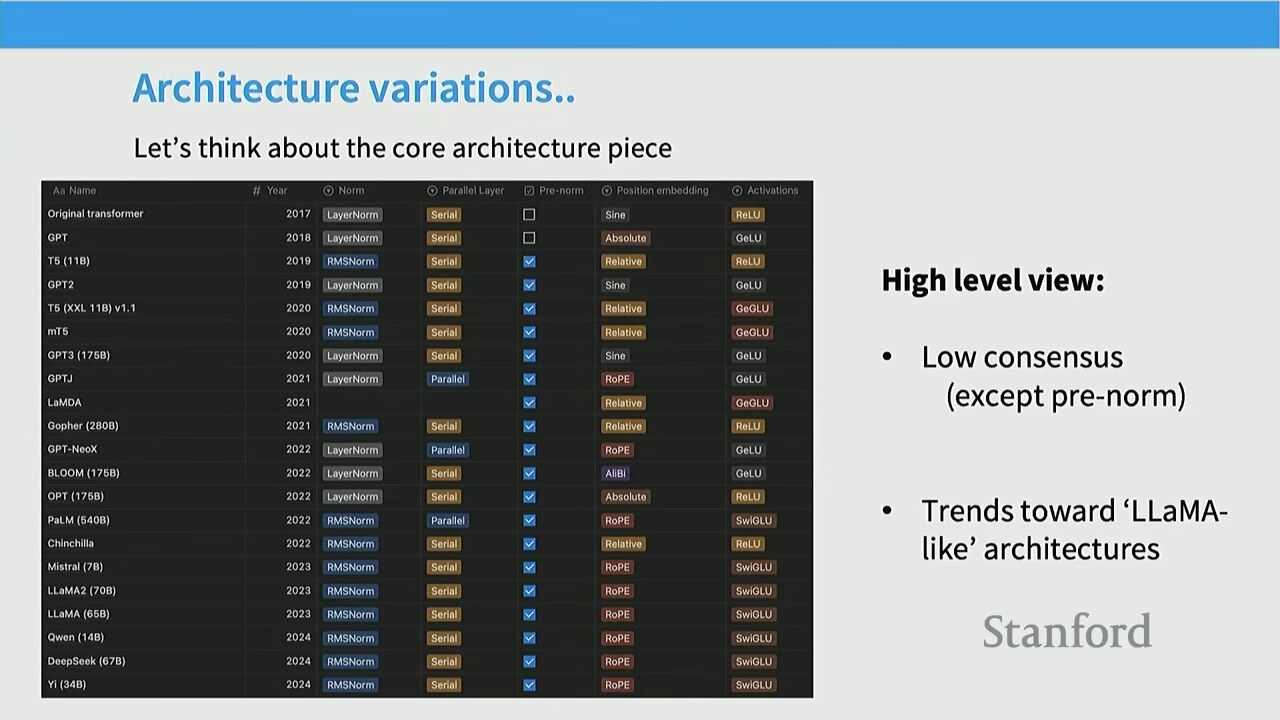
\includegraphics[width=\textwidth]{figures/fig_23_design_questions.jpg}
\caption{设计问题清单：训练 LM 需要决策的所有架构/超参选项一览\protect\footnotemark}
\end{figure}
\footnotetext{视频画面时间区间：00:05:15--00:05:45。}

需要回答的问题包括：FFN 应该多大？多少个 head？词表多大？模型多宽多深？这些我们逐一用证据来约束。

\subsection{FFN 内层维度 $d_{\mathrm{ff}}$：4x 与 8/3x 的约定}

从一个简单的 ReLU FFN 出发，有两个维度超参数：输入维度 $d_{\mathrm{model}}$（残差流宽度）和 FFN 内层隐维度 $d_{\mathrm{ff}}$（上投影后的宽度）。

\begin{figure}[H]
\centering
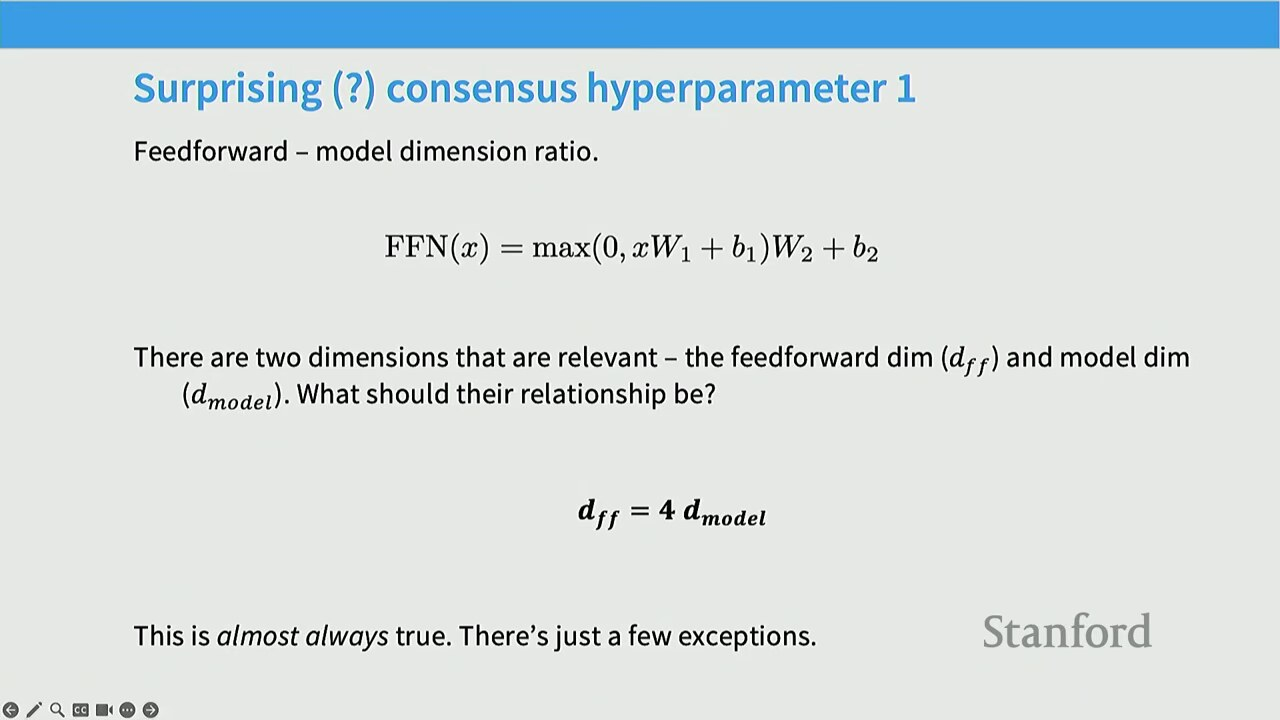
\includegraphics[width=\textwidth]{figures/fig_13_ffn_ratio.jpg}
\caption{FFN 内层维度 $d_{\mathrm{ff}}$ 选择：常见 4× 与 SwiGLU 下的 $(8/3)$×，各模型取值对比\protect\footnotemark}
\end{figure}
\footnotetext{视频画面时间区间：00:42:15--00:42:45。}

\begin{importantbox}{$d_{\mathrm{ff}}$ 的两条约定}
\begin{itemize}
    \item \textbf{非门控（ReLU/GELU）FFN}：几乎所有人都选 $d_{\mathrm{ff}} = 4 \, d_{\mathrm{model}}$。
    \item \textbf{门控（GLU）FFN}：为了与 $4\times$ 版本\emph{参数量匹配}（因为多了一个门控矩阵 $V$），把宽度缩到原来的 $2/3$，即 $d_{\mathrm{ff}} = \tfrac{8}{3} d_{\mathrm{model}} \approx 2.66\, d_{\mathrm{model}}$。
\end{itemize}
\end{importantbox}

推导 $8/3$ 的逻辑：门控 FFN 有三个矩阵（$W_1, V, W_2$），而非门控只有两个（$W_1, W_2$）。设非门控宽度 $d_{\mathrm{ff}}^{(\text{old})} = 4 d$，参数量 $2 \cdot d \cdot 4d = 8d^2$；门控版若宽度为 $d_{\mathrm{ff}}^{(\text{new})}$，参数量 $3 \cdot d \cdot d_{\mathrm{ff}}^{(\text{new})}$。令两者相等：$3 d \cdot d_{\mathrm{ff}}^{(\text{new})} = 8d^2$，解得 $d_{\mathrm{ff}}^{(\text{new})} = \tfrac{8}{3}d$。

Llama、Qwen、DeepSeek-V1、T5 等都大致遵循这个 2.66 规则。Tatsu 特别欣赏一个"叛逆者"——\textbf{T5 11B}：它的 $d_{\mathrm{model}}=1024$，却把 $d_{\mathrm{ff}}$ 设到了惊人的 65536，即 \textbf{64 倍}！T5 的理由是"更宽的矩阵乘能拿到更好的 GPU 并行度"。Gemma 2 也跟风用了 8 倍。这证明规则是可以打破的——但有趣的是，PaLM 的后续版本 PaLMv1.1 把倍数回调到了更标准的 2.5（GeGLU），暗示"也许我们想撤回那个 64× 的激进选择"，而且确实得到了更好的模型。

\subsubsection{Kaplan scaling law 论文里的定量证据}

\begin{figure}[H]
\centering
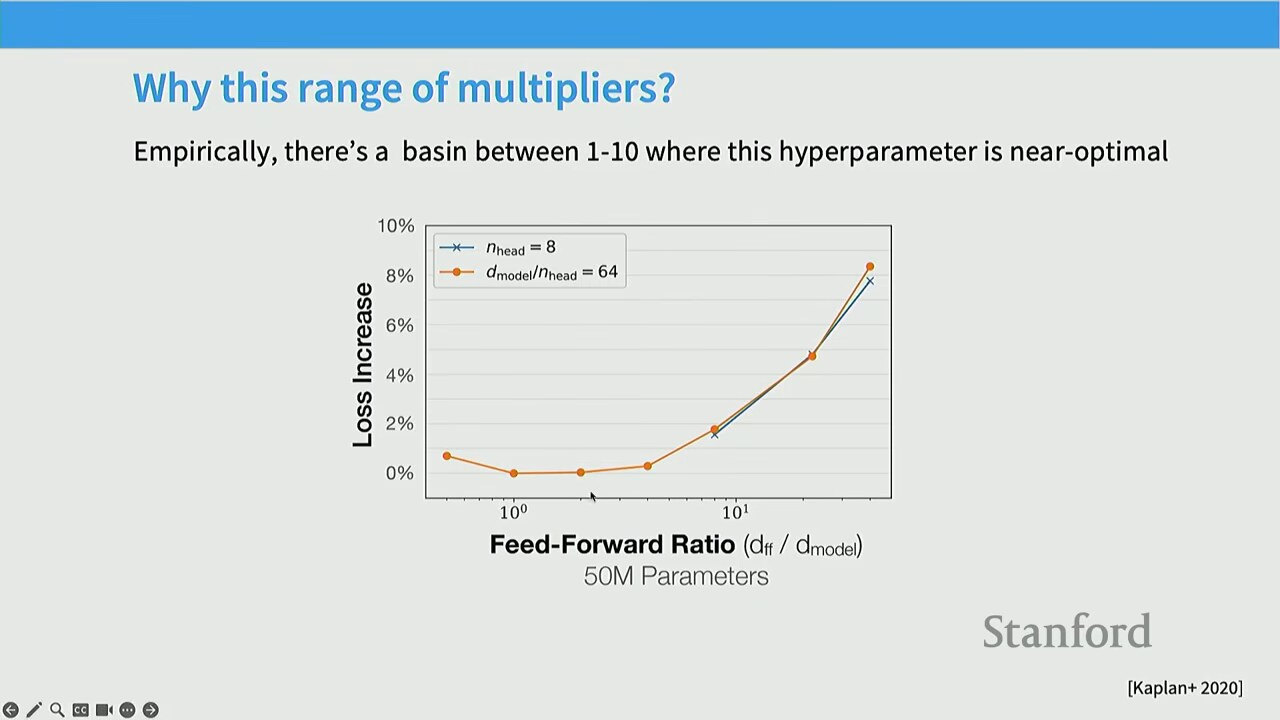
\includegraphics[width=\textwidth]{figures/fig_14_ffn_multiplier_range.jpg}
\caption{FFN 倍数取值范围（1--10）：50M 模型 loss vs FFN ratio 扫描，经验最优区间\protect\footnotemark}
\end{figure}
\footnotetext{视频画面时间区间：00:45:45--00:46:15。}

有没有定量实验支撑"4×"？有——Jared Kaplan 的 scaling law 论文（大家通常只记它的 scaling law 部分，但其实里面有很有用的超参数部分）。他们画了"loss 增量随 $d_{\mathrm{ff}}/d_{\mathrm{model}}$ 比例变化"的曲线：在 1 到 10 之间存在一个相当宽的"甜区"（sweet basin），4 就在最优附近。所以 4 不是"自然定律"，而是一个"convention that has really held up"。

\subsection{Head 维度与数量：保持 $d_{\mathrm{model}} = n_{\mathrm{heads}} \cdot d_{\mathrm{head}}$}

另一个"surprising consensus"：模型维度 $d$ 与"head 数 $\times$ 每 head 维度"的比值。

\begin{importantbox}{head 维度的 1:1 约定}
几乎所有模型都保持 $d_{\mathrm{model}} = n_{\mathrm{heads}} \cdot d_{\mathrm{head}}$，即比值约为 \textbf{1}。换言之，增加 head 数时，每个 head 分到的维度\emph{等比缩小}，而不是保持每 head 维度不变（那样会让 attention 部分吃掉越来越多参数）。

GPT-3、T5、Llama、PaLM、Llama 2 比值都是 1 或接近 1。唯一的叛逆者又是 T5（比值 16）。
\end{importantbox}

有论文（Bogdan Penatti et al. 2020）反对这个 1:1 约定，论证"head 越多，每个 head 的秩越低，会损害 attention 的表达能力"。但实践中似乎并没有看到严重的低秩瓶颈，1:1 的模型表现得很好。

\subsection{宽深比（Aspect Ratio）：约 128 维/层}

\begin{figure}[H]
\centering
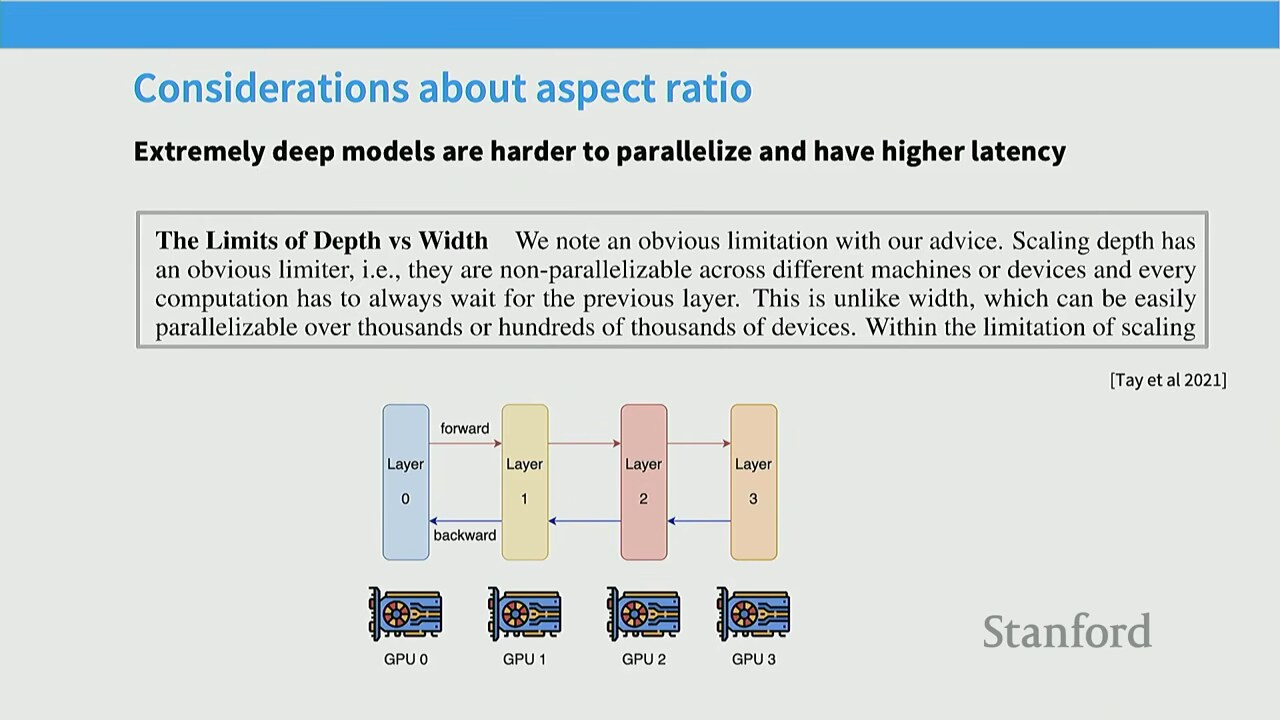
\includegraphics[width=\textwidth]{figures/fig_15_aspect_ratio.jpg}
\caption{深度 vs 宽度（aspect ratio）：深层难并行、延迟高，浅层易并行，trade-off 讨论\protect\footnotemark}
\end{figure}
\footnotetext{视频画面时间区间：00:51:45--00:52:15。}

模型可以做得更深（更多层）或更宽（更大 $d_{\mathrm{model}}$）。控制宽度的主要旋钮是残差流的隐维度 $d_{\mathrm{model}}$。早期模型有的很"矮胖"（宽远大于深），有的很"高瘦"。经验上收敛到一个甜区：\textbf{大约每层 128 个 hidden dimension}——GPT-3 和 Llama 系列大致遵循。

宽深比还牵涉到\textbf{系统层面的并行约束}：

\begin{itemize}
    \item \textbf{Pipeline parallel}：把不同层切到不同设备，需要较深的模型才有意义。
    \item \textbf{Tensor parallel}：把单个大矩阵切片分布到 GPU，需要较宽的模型，且对网络延迟很敏感。
\end{itemize}

所以你的网络拓扑（快/慢、高/低延迟）会反过来约束宽深选择。Kaplan 论文再次提供了定量证据：在 50M / 274M / 1.5B 三个尺度上画 aspect ratio vs loss，\emph{约 100 处都是最低点}，而且最优点在不同尺度间漂移很小——这意味着你可以在一个固定的 aspect ratio 上持续训练。Tay et al.（Google）的一个有趣发现是：看\emph{loss} 时只有参数量重要（深浅无所谓）；但看\emph{下游 fine-tune 准确率}时，同样 FLOPs 下更深可能更好。

\subsection{词表大小：从 3--5 万到 10--25 万}

词表大小呈明显上升趋势。早期单语模型（GPT、早期 Llama）多在 \textbf{30k--50k}；而多语/生产级模型（Command A、GPT-4 系 tokenizer 及其模仿者）已普遍到 \textbf{100k--250k}。原因是 LM 被部署到真实世界，要处理多语言、emoji 等。Cohere 因为强调多语，词表特别大。对低资源语言，大词表能把它们的文本"pack"进更少的 token，降低推理成本。

可以用一个简单的"压缩比"来度量词表效率：

\[
\rho = \frac{\text{原生字符数}}{\text{token 数}}
\]

\begin{itemize}
    \item $\rho$：平均每个 token 承载的字符数（compression ratio）。
    \item 对英语，$\rho$ 通常约 4；对低资源语言，小词表会让 $\rho$ 显著下降（每个 token 只覆盖 1--2 个字符），推理与训练成本暴涨。
    \item 大词表（如 Cohere）把低资源语言的 $\rho$ 拉高，使推理时"pay much fewer tokens"——这是多语词表的核心收益。
\end{itemize}

\subsection{上下文长度：训练窗口与外推}

\begin{figure}[H]
\centering
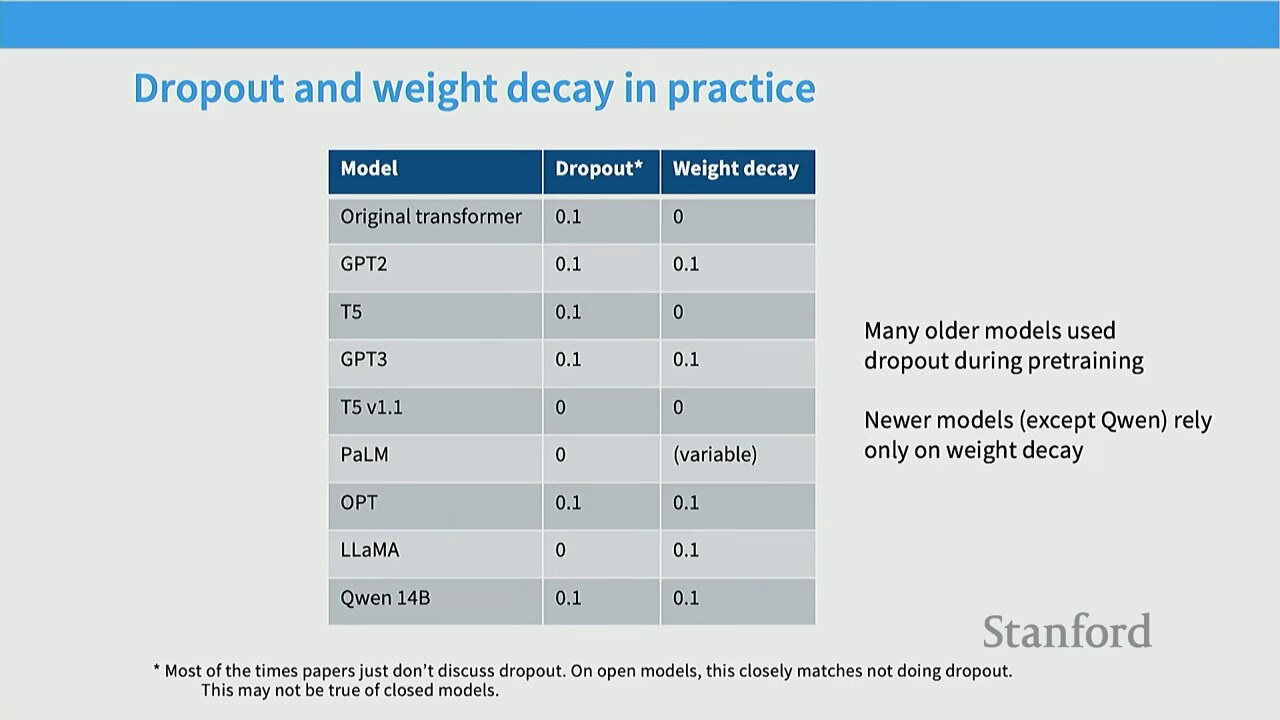
\includegraphics[width=\textwidth]{figures/fig_16_context_length.jpg}
\caption{上下文长度选择：各模型 context window 大小与长上下文带来的训练/外推 trade-off\protect\footnotemark}
\end{figure}
\footnotetext{视频画面时间区间：00:57:45--00:58:15。}

上下文长度（训练时用的序列窗口）也是一个关键超参，且呈增长趋势。它与两个问题挂钩：(1) 训练成本随上下文二次增长（attention 是 $O(N^2)$）；(2) 测试时若要超出训练长度，需要专门的外推技巧（这也是 RoPE 生态繁荣的原因——它衍生出大量长度外推算法）。Llama 4 等最新模型通过混合稀疏注意力（见后文）宣称支持千万级 token 上下文。

Attention 的序列长度代价可定量写成：

\[
\mathrm{FLOPs}_{\text{attn}} \propto B \cdot N^2 \cdot d_{\mathrm{head}} \cdot n_{\mathrm{heads}}
\]

\begin{itemize}
    \item $N^2$：attention 矩阵的尺寸（每个 token attend 所有 token）。
    \item 这就是为什么 sliding window / sparse attention 把 $N^2$ 降到 $N \cdot w$（$w$ 为窗口大小）能带来巨大节省。
\end{itemize}

\subsection{初始化与 muP：让超参数可迁移}

\begin{figure}[H]
\centering
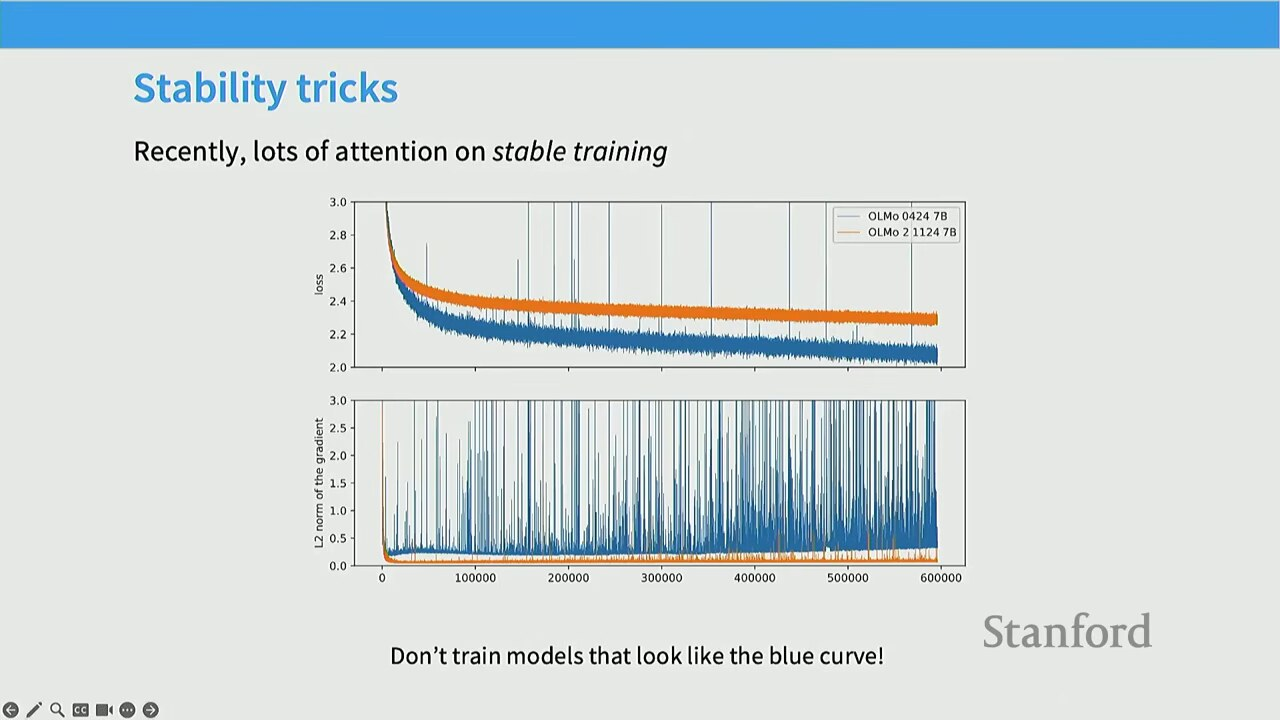
\includegraphics[width=\textwidth]{figures/fig_17_init_mup.jpg}
\caption{初始化与 muP：Xavier/He 初始化 + maximal update parameterization 实现超参迁移\protect\footnotemark}
\end{figure}
\footnotetext{视频画面时间区间：01:05:45--01:06:15。}

权重初始化直接影响训练能否起步。最常见的是 \textbf{Xavier/Glorot} 初始化（适配 tanh/sigmoid 的均匀分布）与 \textbf{He/Kaiming} 初始化（适配 ReLU 族）。核心思想是让各层激活与梯度的方差保持稳定：

\[
\text{Xavier:} \quad \mathrm{Var}(W_{ij}) = \frac{2}{n_{\mathrm{in}} + n_{\mathrm{out}}}
\qquad
\text{He:} \quad \mathrm{Var}(W_{ij}) = \frac{2}{n_{\mathrm{in}}}
\]

\begin{itemize}
    \item $n_{\mathrm{in}}, n_{\mathrm{out}}$：该层权重的输入/输出维度（fan-in / fan-out）。
    \item 目标：前向传播时激活方差不变，反向传播时梯度方差不变，避免深层网络的"消失/爆炸"。
\end{itemize}

\textbf{muP（Maximal Update Parameterization）}解决的是更深层的问题：\emph{如何把小模型上调好的超参数（尤其是学习率）迁移到大模型}。标准参数化（standard parameterization, SP）下，不同宽度的模型最优学习率不同，每次放大都要重新调参；muP 通过精心设计各层权重与学习率的缩放，使得\emph{模型变宽时每一层的激活更新幅度保持不变}：

\[
\Delta h_{\ell} \approx \text{常数（与宽度无关）} \quad \text{在 muP 下}
\]

\begin{itemize}
    \item $\Delta h_{\ell}$：第 $\ell$ 层激活在一次更新中的变化幅度。
    \item 这让你可以在小模型上扫描学习率等超参，再把最优值直接搬到大模型上，节省海量调参算力。
\end{itemize}

\begin{practicebox}{超参数的"无需深思"清单}
Tatsu 总结：以下超参基本是 no-brainer，已被反复验证，照做即可——FFN 隐层大小（4× 或 2.66×）、head 维度、aspect ratio（~128/层）、weight decay 做正则。作业里建议的默认值大致就对应这些共识。
\end{practicebox}

\subsection{正则化：Dropout 退场，Weight Decay 留下的悖论}

正则化这一节有一个"intuition-violating"（违反直觉）的精彩讨论。预训练通常是\textbf{单 epoch}、数据多到训不完，根本不可能过拟合——那为什么还要正则化？

\begin{itemize}
    \item \textbf{Dropout}：早期很流行，现在已经\emph{过时}。Tatsu 没见过任何结果显示 dropout 对训练 loss 有帮助，而逻辑上也确实不存在单 epoch 下的过拟合问题。
    \item \textbf{Weight decay}：反而保留了下来，且几乎所有大模型都在用。这很反直觉。
\end{itemize}

为什么预训练要用 weight decay？答案令人意外：\textbf{不是为了控制过拟合}（不同 weight decay 强度下，train/val loss gap 几乎不变），而是因为它与\emph{学习率调度}有复杂的交互，能在训练尾部带来更低的训练 loss。

标准的 weight decay 更新（L2 正则）与 cosine learning rate schedule 写成：

\[
w_{t+1} = (1 - \lambda) w_t - \eta_t \, \nabla \mathcal{L}(w_t), \qquad
\eta_t = \eta_{\min} + \tfrac{1}{2}(\eta_{\max} - \eta_{\min})\left(1 + \cos\!\left(\tfrac{t}{T}\pi\right)\right)
\]

\begin{itemize}
    \item $\lambda$：weight decay 系数（每步把权重乘以 $1-\lambda$）。
    \item $\eta_t$：第 $t$ 步的学习率，按 cosine 从 $\eta_{\max}$ 衰减到 $\eta_{\min}$，$T$ 为总步数。
    \item 关键交互：在 cosine 尾部 $\eta_t \to \eta_{\min}$（通常为 0）时，高 $\lambda$ 的模型会"非常迅速地"优化——这是隐式加速的来源。
\end{itemize}

\begin{warningbox}{Weight decay 的真实作用：与学习率尾部的隐式加速}
观察到的现象：在常数学习率下，高 weight decay 的模型训练得慢；但当学习率突然下降（cosine decay 的尾部）时，它会\emph{非常迅速}地优化、loss 急剧下降。也就是说，weight decay 在学习率冷却阶段触发了一种"implicit acceleration"，最终给出\emph{更好的训练 loss}（而训练 loss 与 val loss 又几乎相同）。

所以你不是为了正则化而 weight decay，而是为了\emph{拿到更低的训练 loss}——这正是我们要优化的目标。这是一个"troubling but real"的经验事实。
\end{warningbox}

\section{训练稳定性技巧：过去一年的新主题}

Tatsu 在普查新论文时发现：\textbf{核心架构其实没怎么变，但"stability tricks"（稳定性技巧）被前所未有地强调}。随着模型变大、训练变长，loss spike 和梯度爆炸问题越来越频繁。

OLMo 2 论文里有一张"恐怖"的图：loss 曲线看起来还好，但打开梯度 L2 norm，会发现到处是爆炸性的 spike——这种训练随时可能"hit, gradient norm explodes, training is done"。目标就是把蓝色的锯齿曲线变成橙色的平滑曲线。

\subsection{问题根源：Softmax 的数值不稳定性}

稳定性问题在 Transformer 里\emph{到处}都可能出现，但有一个"problem child"（问题儿童）格外突出：\textbf{softmax}。它要取指数（可能数值爆炸）、要做除法（可能除以零）。Transformer 里有两个 softmax 需要处理：(1) 输出层的 output softmax；(2) self-attention 里的 attention softmax。

\subsection{Z-loss：稳定输出 Softmax}

\begin{figure}[H]
\centering
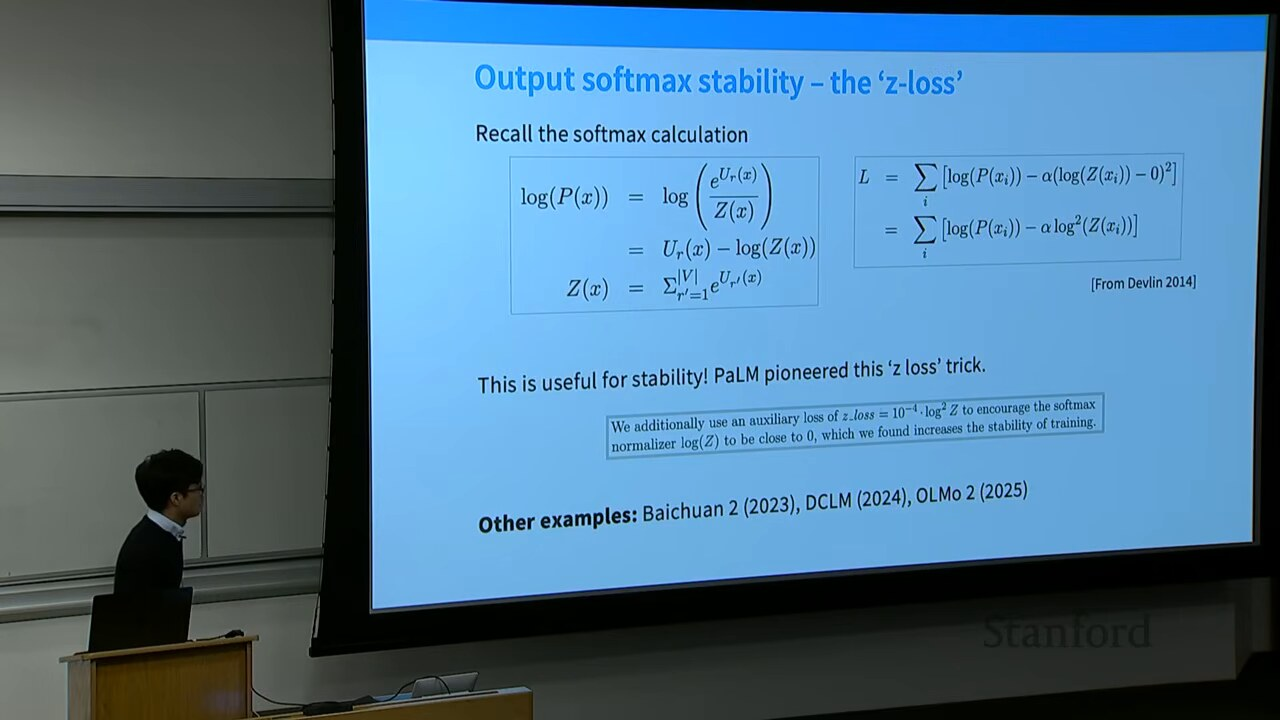
\includegraphics[width=\textwidth]{figures/fig_18_z_loss.jpg}
\caption{Output softmax 稳定性：PaLM 的 z-loss 技巧，约束 softmax 归一化项 $\log Z \approx 0$\protect\footnotemark}
\end{figure}
\footnotetext{视频画面时间区间：01:09:45--01:10:15。}

第一个技巧叫 \textbf{z-loss}，最早可追溯到 Devlin 2014 的机器翻译论文（动机完全不同），但在 LM 领域是 \textbf{PaLM} 首倡。输出 softmax 写成：

\[
p(x) = \frac{\exp(u(x))}{Z(x)}, \qquad Z(x) = \sum_{x'} \exp(u(x'))
\]

\begin{itemize}
    \item $u(x)$：token $x$ 的 logit。
    \item $Z(x)$：softmax 的归一化项（partition function），对所有词表项求 exp 之和。
\end{itemize}

我们希望 $Z(x)$ 接近 1（即 $\log Z(x) \approx 0$），这样 $\exp/\text{除法}$ 都数值友好。于是加一个辅助损失项：

\[
\mathcal{L}_{\text{aux}} = \alpha \cdot \big(\log Z(x)\big)^2
\]

\begin{itemize}
    \item $\alpha$：小权重（PaLM 用 $\alpha = 10^{-4}$）。
    \item $(\log Z(x))^2$：惩罚 $\log Z$ 偏离 0。
\end{itemize}

如果成功，$\log Z \to 0$ 则 $\exp$ 与 $\log$ 抵消，softmax 退化为干净的 logit 操作，所有"problematic operations"消失。PaLM 之后，Baichuan 2、DCLM、OLMo 2 等纷纷采用 z-loss。

\subsection{QK Norm：稳定 Attention Softmax}

第二个 softmax 在 attention 里。技巧叫 \textbf{QK norm}：在算 $Q K^\top$ \emph{之前}，先把 query 和 key 各自过一个 layer norm。

\[
\text{原 attention logits:} \quad Q K^\top
\qquad
\text{QK norm:} \quad \mathrm{LN}(Q)\,\mathrm{LN}(K)^\top
\]

\begin{itemize}
    \item 这里不是控制归一化项 $Z$，而是\emph{控制 softmax 的输入}让其有界，从而间接控制 softmax 的不良行为。
    \item 这个技巧源自\textbf{视觉/多模态}社区（Dehghani 2023 训练大型 ViT；Chameleon、HuggingFace 的 Edith Feix 用于多模态），后来才"seeped back"到纯文本 LM 训练。Gemma 2、DCLM、OLMo 2 都用了。
\end{itemize}

\subsection{Soft Capping：对 Logits 做 tanh 软裁剪}

第三个技巧不那么常用：对 attention logits 做\textbf{软裁剪}（soft cap）。

\[
\text{softcapped logits} = \frac{\mathrm{tanh}(\text{logits} / \tau) \cdot \tau}{}
\]

\begin{itemize}
    \item $\tau$：soft cap 阈值。
    \item $\mathrm{tanh}$ 把超过 $\tau$ 很多的 logits 裁到 1，使最大值不超过 $\tau$。
\end{itemize}

Gemma 2 用了这个技巧。但 NVIDIA 的消融显示它\emph{反而让 perplexity 变差}（11.19 → 更高），而 QK norm 因为允许更激进的学习率，反而让 perplexity 更好。

\begin{knowledgebox}{Layer norm 的"无处不在"——一个稳定性奇迹}
Tatsu 在这一节的总结里只允许自己讲一个笑话：layer norm 作为稳定性干预\emph{shockingly effective}（惊人地有效）。从只在 pre-norm 位置，到 block 前后都放（double norm），再到塞进 Q 和 K（QK norm）——layer norm 在"几乎不影响性能的前提下极大提升稳定性"这件事上，表现始终令人惊叹。
\end{knowledgebox}

有学生问：QK norm 在\emph{推理时}还保留吗？Tatsu：当然保留。layer norm 已经学到了把激活归一化到特定 scale 的参数，推理时拿掉它会让模型面对未归一化的激活"have no idea what to do"，是灾难性的改变。

\section{注意力变体与推理效率}

最后一节（如果时间允许）讲注意力 head 的变体。Tatsu 强调这些"对训练时行为不太关键，但对\emph{推理成本与行为}至关重要"。

\subsection{为什么自回归生成慢？KV Cache}

\begin{figure}[H]
\centering
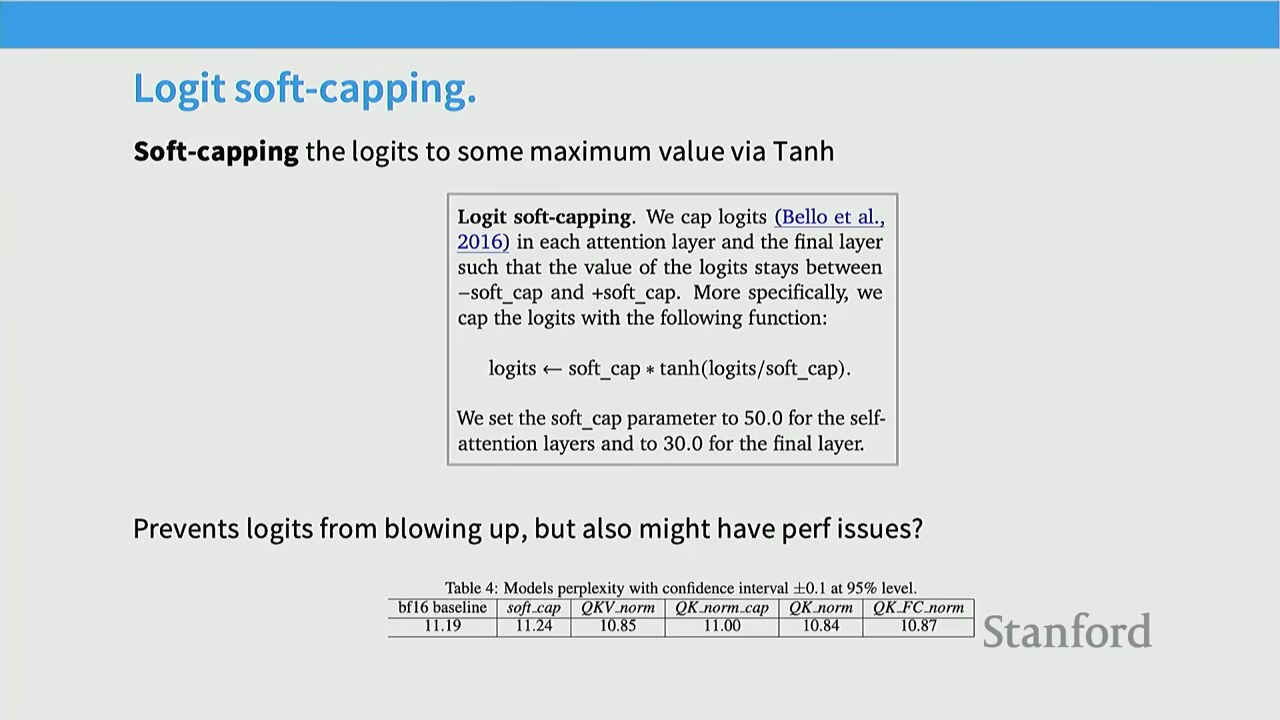
\includegraphics[width=\textwidth]{figures/fig_19_kv_cache_slow.jpg}
\caption{为何自回归生成慢：decode 阶段逐 token、memory-bound，引出 KV cache\protect\footnotemark}
\end{figure}
\footnotetext{视频画面时间区间：01:14:45--01:15:15。}

训练时我们有大的 batch 矩阵可以并行乘，arithmetic intensity（每次内存访问对应的计算量）很高。但推理（生成）时是\textbf{逐 token 自回归}：生成一个 token，喂回去，再生成下一个，无法并行。这就引出了 \textbf{KV cache}。

\begin{figure}[H]
\centering
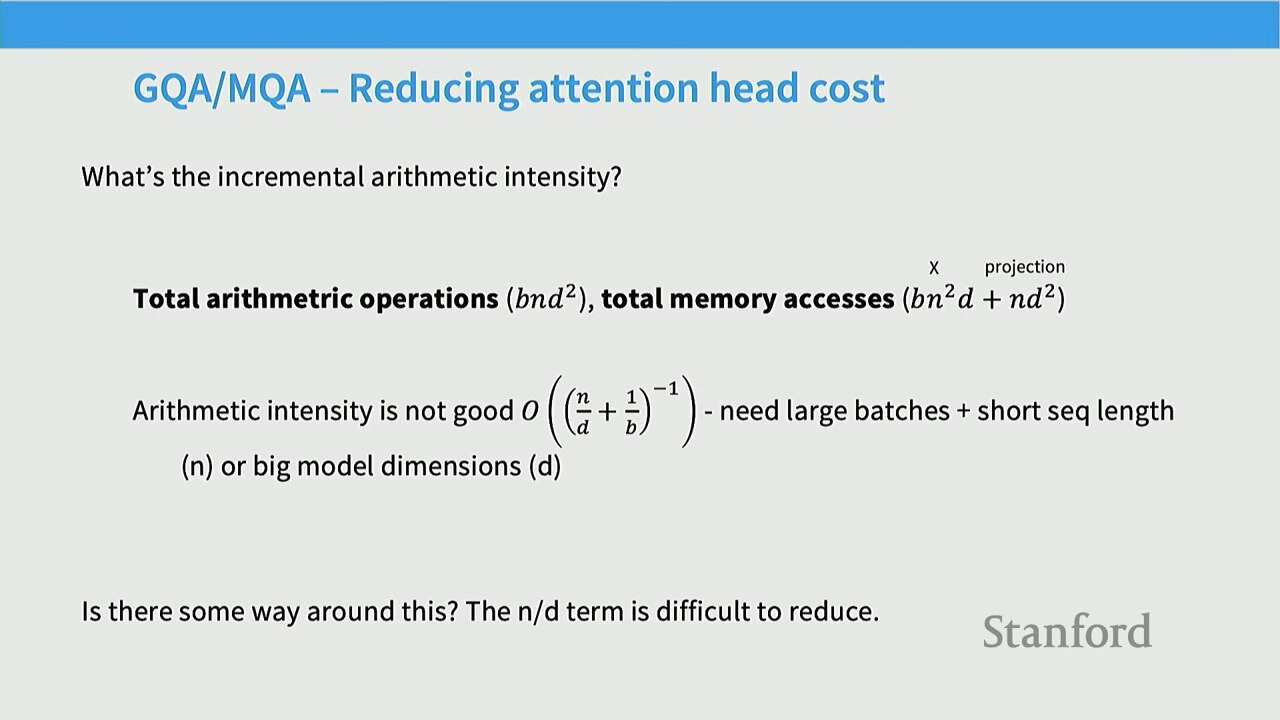
\includegraphics[width=\textwidth]{figures/fig_25_kv_cache_memory.jpg}
\caption{KV cache 内存开销：随序列长度线性增长，长上下文推理的主要瓶颈\protect\footnotemark}
\end{figure}
\footnotetext{视频画面时间区间：01:20:45--01:21:15。}

KV cache 的核心思想：每生成一个新 token，它的 query 是新的，但\emph{过去所有 token 的 key 和 value 都不变}（它们只依赖过去）。所以把过去的 K、V \emph{缓存}起来，增量地追加新 token 的 K、V，每次只算新 query 与缓存里所有 key 的一行内积（下三角 attention 矩阵的一行）。这避免了重复计算，但代价是\textbf{内存搬运量急剧上升}。

\subsection{Arithmetic Intensity：训练 vs 推理}

\begin{figure}[H]
\centering
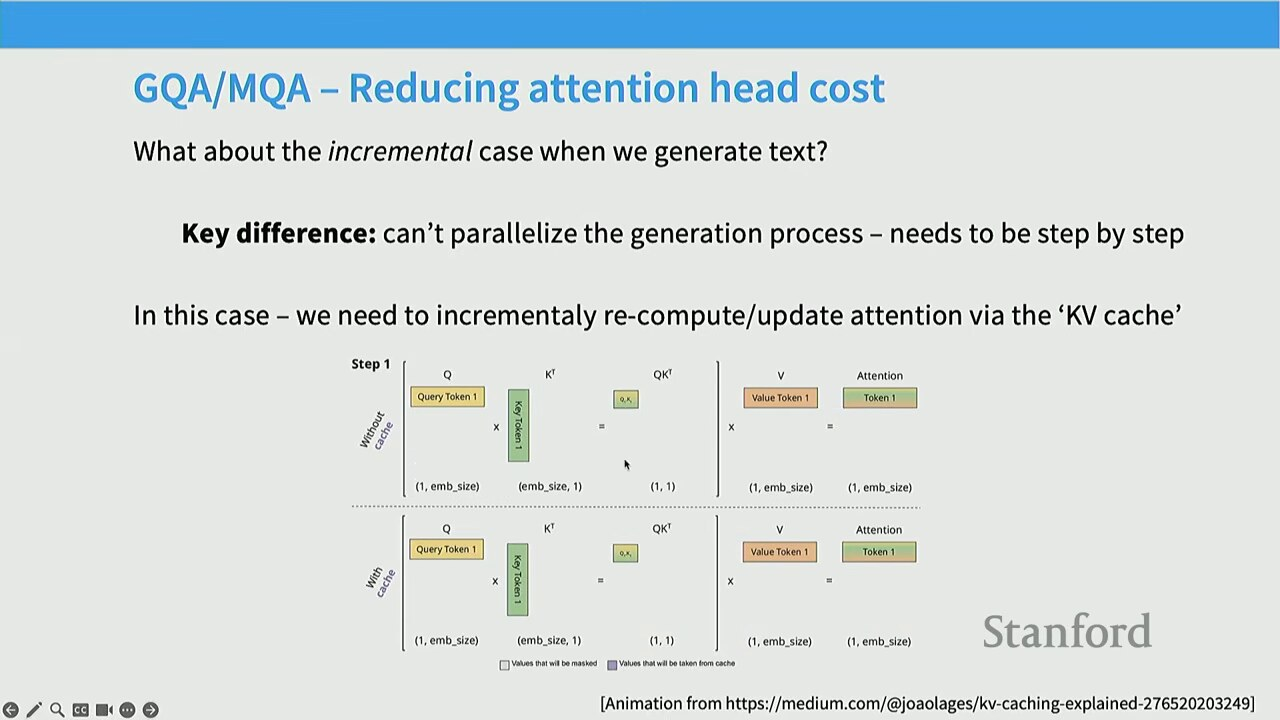
\includegraphics[width=\textwidth]{figures/fig_20_arithmetic_intensity.jpg}
\caption{Arithmetic intensity（FLOPs/byte）：prefill compute-bound vs decode memory-bound 的 roofline 分析\protect\footnotemark}
\end{figure}
\footnotetext{视频画面时间区间：01:20:15--01:20:45。}

Tatsu 算了一笔账。Attention 的总算术操作量约为 $B \cdot N \cdot D^2$（$B$=batch，$N$=序列长，$D$=隐维度）。

\textbf{训练 / prefill}（大 batch）：
\[
\text{arithmetic intensity} \approx \frac{\text{FLOPs}}{\text{mem access}} \approx \frac{1}{1/H + 1/(BN)} \quad\text{（很高，compute-bound）}
\]

\begin{itemize}
    \item $H$：head 数。$BN$ 大时第二项可忽略，强度 $\approx H$，很高。
    \item 大 batch、长序列、多 head 都让 GPU 保持在 compute-bound 区间。
\end{itemize}

\textbf{推理 / decode}（逐 token，KV cache）：
\[
\text{arithmetic intensity} \approx \frac{1}{N/D + 1/B}
\]

\begin{itemize}
    \item 现在 $N/D$ 这一项\emph{很糟糕}：要强度高，需要 $N/D$ 小（短序列或大模型）和 $B$ 大——但我们既不想要更大的模型，也不想要更短的序列。
    \item 这就是推理吞吐的核心 trade-off：\textbf{memory-bound}，被 $N/D$ 这一项"杀死"。
\end{itemize}

\begin{warningbox}{推理的真正瓶颈：内存搬运，不是计算}
decode 阶段算术强度低意味着 GPU 大部分时间在\emph{等内存}。每次用 K 矩阵做乘法，都要把 K 从内存搬到计算单元，算完再搬走、算激活、再搬回来……这种反复的内存搬运让总内存访问量膨胀到 $B^2 D + N D^2$。计算量没变（$BND$），但内存访问暴增——这就是 decode 慢的根因。
\end{warningbox}

\subsection{MQA 与 GQA：共享 Key/Value 头}

\begin{figure}[H]
\centering
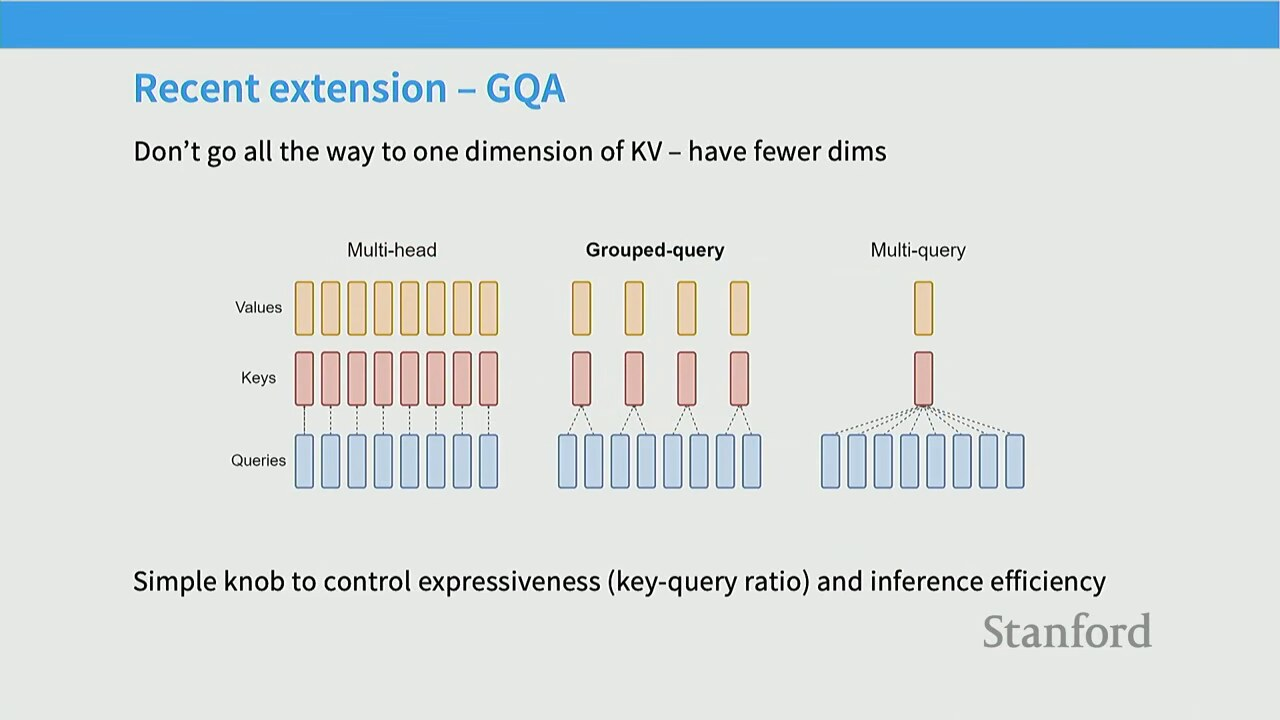
\includegraphics[width=\textwidth]{figures/fig_21_attention_variants.jpg}
\caption{注意力变体：MHA / MQA / GQA / MLA，key/value head 如何在 query head 间共享\protect\footnotemark}
\end{figure}
\footnotetext{视频画面时间区间：01:23:45--01:24:15。}

既然瓶颈是 K、V 的搬运，那\textbf{减少 K、V 的头数}就能直接缓解。\textbf{Multi-Query Attention (MQA)} 的做法：query 仍然有多个 head，但\emph{所有 query head 共享同一个 K head 和一个 V head}。这样 K、V 的搬运量大幅下降，arithmetic intensity 改善——第一项除以了 $N$（更长序列变得可行），第二项除以了 head 数。

\textbf{Grouped-Query Attention (GQA)} 是 MQA 的折中：不是所有 query 共享 1 个 K/V，而是分成若干组，每组共享一个 K/V。这样在"推理效率"与"模型表达力"之间做 trade-off——从 MHA 一路降到 MQA 可能太激进，GQA 给了中间档。有工作显示 GQA 不掉点而 MQA 会。

\begin{importantbox}{MHA / MQA / GQA 一句话总结}
\begin{itemize}
    \item \textbf{MHA}（标准多头）：每个 query head 有自己的 K、V head。表达力最强，但 KV cache 最大。
    \item \textbf{MQA}：所有 query head 共享 1 个 K、V head。KV cache 最小，但可能损害质量。
    \item \textbf{GQA}：query head 分组，组内共享 K、V head。质量与效率的甜区，现代大模型（Llama 等）的主流选择。
\end{itemize}
\end{importantbox}

KV cache 的内存占用直接受 K/V 头数控制：

\[
\text{Mem}_{\text{KV}} = 2 \cdot n_{\text{kv\_heads}} \cdot N \cdot d_{\text{head}} \cdot \text{(每参数字节数)}
\]

\begin{itemize}
    \item $n_{\text{kv\_heads}}$：K/V 的头数。MHA 下 $= n_{\text{heads}}$；MQA 下 $= 1$；GQA 介于之间。
    \item 系数 2：同时缓存 K 和 V。
    \item 从 MHA 到 MQA，$n_{\text{kv\_heads}}$ 从 $n_{\text{heads}}$ 降到 1，KV cache 内存随比例下降——这就是 MQA/GQA 改善 decode arithmetic intensity 的根源。
\end{itemize}

\subsection{稀疏与滑动窗口注意力：通往超长上下文}

最后，Tatsu 提到如何支持超长上下文（如 Llama 4 号称 1000 万 token）。OpenAI 2019 的 Sparse Transformer 提出\textbf{稀疏注意力模式}：不 attend 整个序列，而是只 attend 局部窗口 + 一些对角线模式来跨段传播信息。GPT-3 原始发布就用了这类技巧。\textbf{Sliding window attention}（滑动窗口）是其中一种：每层只 attend 当前位置附近的小窗口，有效感受野 = 窗口大小 $\times$ 层数。

滑动窗口与全注意力的成本对比：

\[
\text{Full:} \quad O(N^2) \quad\text{vs}\quad \text{Sliding window:} \quad O(N \cdot w)
\]

\begin{itemize}
    \item $N$：序列长度，$w$：窗口大小（通常远小于 $N$）。
    \item 全注意力的 $N^2$ 矩阵被替换为带宽 $w$ 的带状矩阵，KV cache 与计算量都大幅下降。
    \item 堆叠 $L$ 层 sliding window 后，有效感受野 $= w \cdot L$，可覆盖远超单层窗口的距离。
\end{itemize}

\begin{practicebox}{Llama 4 / Gemma / Command A 的"混合块"新技巧}
最新的超长上下文技巧（最近几个月）：把若干个（如 4 个）transformer block 组成一组，其中\textbf{最底层那个 block 用 full self-attention + 无位置编码}（既无 RoPE 也无其他），只在每 4 个 block 里出现一次；上面 3 个 block 用\textbf{sliding window attention + RoPE}。

这个设计极其巧妙：(1) 系统层面——full attention 稀疏出现，控制了开销；(2) 长度外推层面——RoPE 只处理局部上下文窗口，而真正超长程的信息走那条\emph{无位置编码}的 full attention 通路，可以"extrapolate very aggressively"，因为根本没有位置编码需要外推。这是近期最酷的发展之一。
\end{practicebox}

\section{总结与延伸}

\begin{figure}[H]
\centering
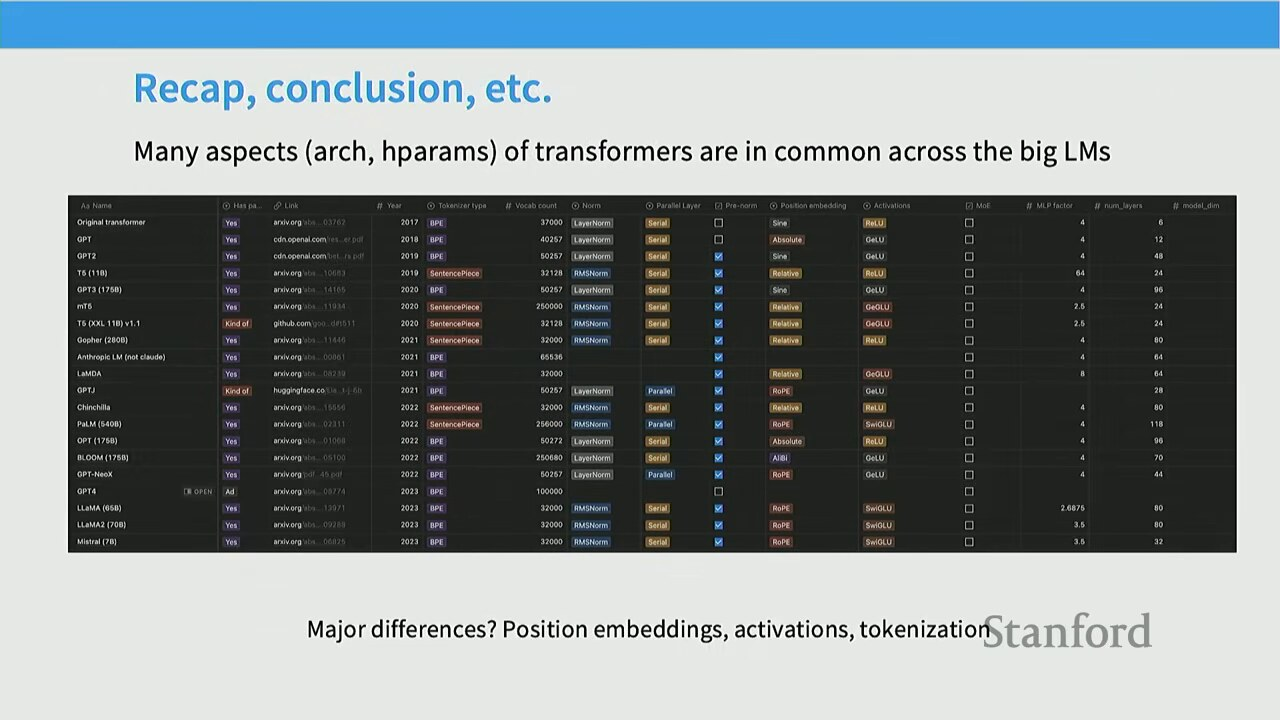
\includegraphics[width=\textwidth]{figures/fig_22_summary.jpg}
\caption{课程总结：回顾本讲要点（架构组件 + 超参选择 + 推理效率）\protect\footnotemark}
\end{figure}
\footnotetext{视频画面时间区间：01:26:45--01:27:00。}

\subsection{本讲核心要点回顾}

本讲以"从他人的经验中学习"为方法论，用一张横跨 2017--2025 的模型普查表，提炼出了现代 Transformer 的设计共识与争议：

\begin{knowledgebox}{可推广的架构教训（Tatsu 的总结）}
\begin{enumerate}
    \item \textbf{直接的恒等残差映射}：让残差流保持纯净的 identity 通路，不要把 norm 塞进去。这条经验在多种架构族里都成立。
    \item \textbf{不让激活在 scale 上漂移}：norm（LayerNorm / RMSNorm）对训练稳定性极其有效，而且"layer norm is shockingly effective"——从 pre-norm 到 double norm 再到 QK norm，反复被验证。
    \item \textbf{门控（gating）}：SwiGLU 等 GLU 变体稳定地带来小幅提升，是继残差、norm 之后的第三条可推广经验。
    \item \textbf{系统视角不可或缺}：FLOPs 不是唯一指标，内存搬运同样（甚至更）重要——RMSNorm、去 bias、并行层、MQA/GQA 都是这条原则的体现。
\end{enumerate}
\end{knowledgebox}

\begin{importantbox}{现代共识 LM 的"标准配方"}
如果你今天要从零训一个 LM，大致照下面选就不会错：
\begin{itemize}
    \item \textbf{Norm}：pre-norm（或 double norm），用 RMSNorm，去掉 bias。
    \item \textbf{激活}：SwiGLU，$d_{\mathrm{ff}} = \tfrac{8}{3} d_{\mathrm{model}}$（参数匹配的 2.66×）。
    \item \textbf{位置编码}：RoPE，作用在 attention 层的 Q/K 上。
    \item \textbf{Head}：保持 $d_{\mathrm{model}} = n_{\mathrm{heads}} \cdot d_{\mathrm{head}}$。
    \item \textbf{宽深比}：约 128 维/层。
    \item \textbf{词表}：100k--250k（多语/生产级）。
    \item \textbf{稳定性}：z-loss + QK norm。
    \item \textbf{推理效率}：GQA 共享 K/V 头。
\end{itemize}
\end{importantbox}

\subsection{留待后续的问题}

本讲刻意把"细节"拉满，但还有几个开放方向：(1) aspect ratio 在\emph{下游任务}（而非 loss）上的最优可能与上游不同（Tay et al. 的发现）；(2) 多模态模型的架构选择（往往是后期 fusion、bolt-on 视觉编码器，但带来了新的稳定性挑战）；(3) 下一讲将深入 DeepSeek-V3 等最新架构。Tatsu 在结尾鼓励大家带着架构与超参的问题来找他——"I'll be happy to answer questions after."

\begin{practicebox}{动手建议}
本讲的所有"共识"都可以在你的 Assignment 实现中亲手验证。当你实现 pre-norm、RoPE、SwiGLU、无 bias 的现代变体时，不要把它们当成"奇怪的强制要求"，而要理解每一处改动背后都有文献与消融支撑。一个很好的练习是：用 Kaplan 论文里的扫描方法，在你自己的小模型上重做 $d_{\mathrm{ff}}/d_{\mathrm{model}}$ 的甜区实验，亲眼看那个 1--10 的宽盆地。
\end{practicebox}

\end{document}
